\section{Ανάλυση Χρονοσειρώ θέσης}
 
\graphicspath{{Chapter2/Figs/}}

 % ------------------------------------------------------------------------------
\begin{frame}
  \frametitle{Εκτίμηση συντεταγμένων - Αρχεία αποτελεσμάτων}
  \framesubtitle{}
  \label{}
  \begin{columns}[T]
    \begin{column}{.5\textwidth}
       
    \end{column}
    \begin{column}{.5\textwidth}
      
    \end{column}
  \end{columns}
\end{frame}
\note{}

 % ------------------------------------------------------------------------------
\begin{frame}
  \frametitle{Ανάλυση χρονοσειρών θέσης}
  \framesubtitle{Πρόγραμμα - παράμετροι}
  \label{}
  \begin{columns}[T]
    \begin{column}{.5\textwidth}
      Ανάλυση χρονοσειρών θέσης με το λογισμικό πακέτο Hector \citep{Bos2012}
      \begin{itemize}\setlength\itemsep{1em}
        \item Τεκτονικές ταχύητες (γραμμικό μοντέλο)
        \item offsets/jupmps: κυρίως λόγο επίδρασης σεισμών καθώς δεν υπάρχουν αλλαγές στον εξοπλισμό.
        \item Αρμονικά σήματα
        \item Αλλαγές ταχυτήτων (πχ. Σαντορίνη)
        \item Μετα-σεισμική παραμόρφωση
      \end{itemize}
    \end{column}
    \begin{column}{.5\textwidth}
      
    \end{column}
  \end{columns}
\end{frame}
\note{}


 % ------------------------------------------------------------------------------
\begin{frame}
  \frametitle{Απομάκρυνση χονδροειδών σφαλμάτων - outliers}
  \framesubtitle{}
  \label{}
  
\end{frame}
\note{}

 % ------------------------------------------------------------------------------
\begin{frame}
  \frametitle{Προσδιορισμός ασυνεχειών - offsets}
  \framesubtitle{}
  \label{}
  \vskip-1cm
  \begin{columns}[T]
    \begin{column}{.33\textwidth}
      \begin{center}
      Station:\textbf{040A}\\
         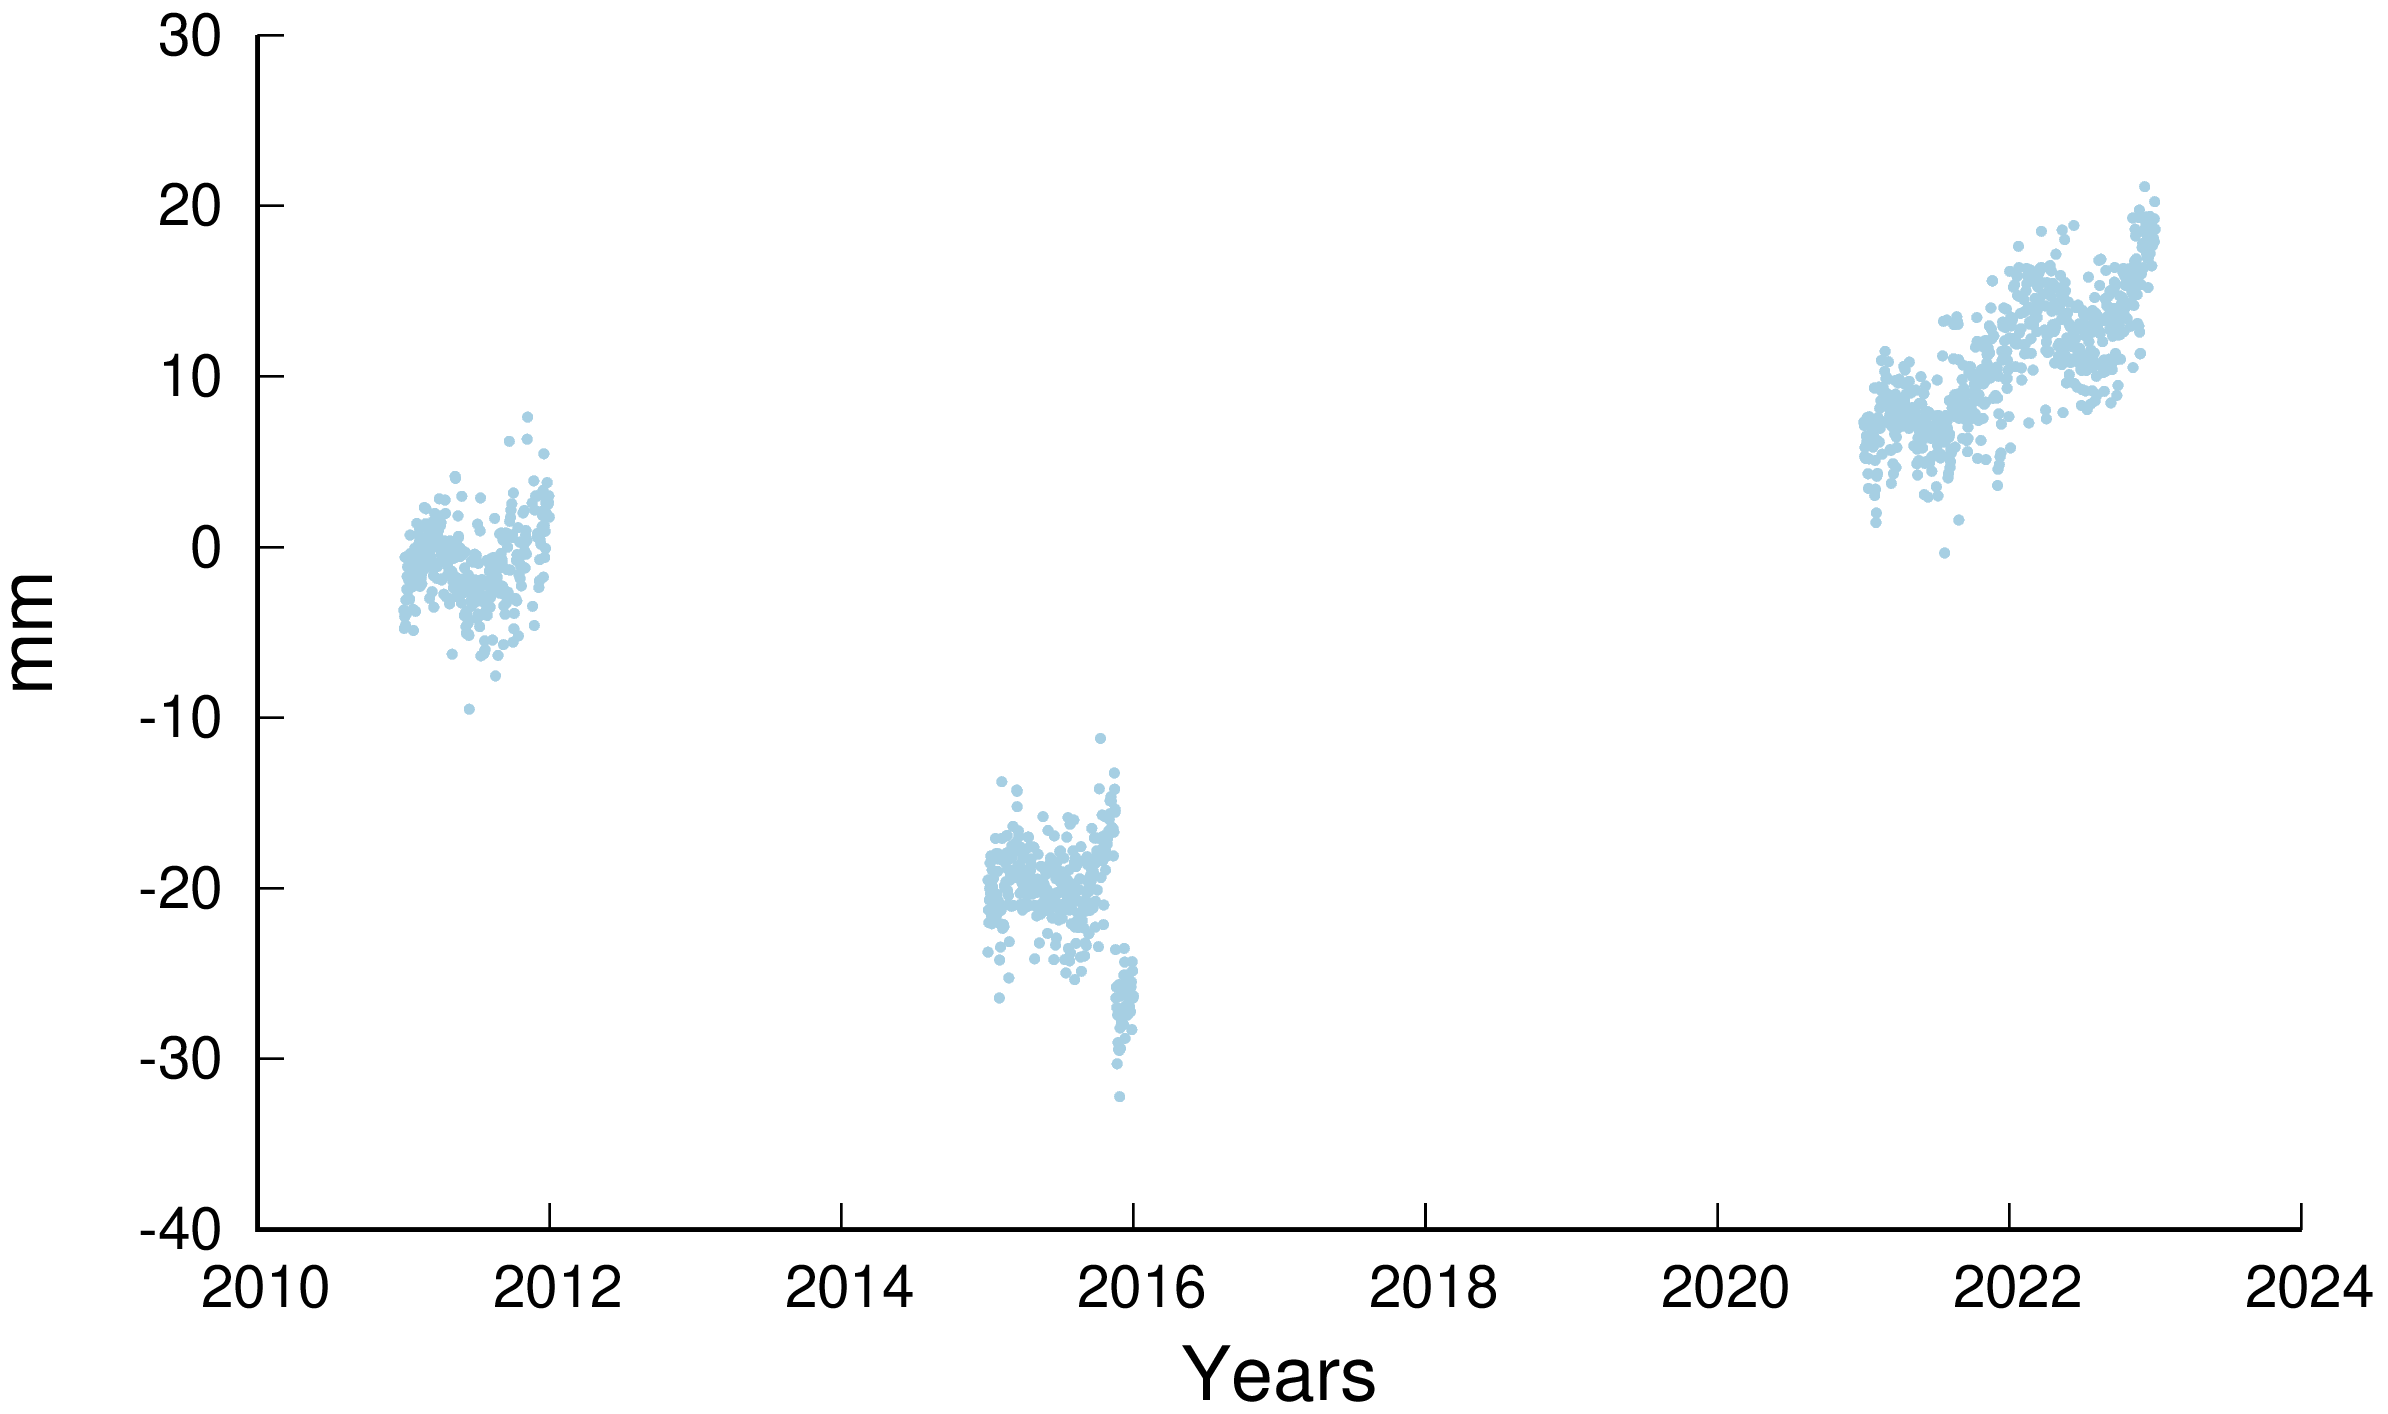
\includegraphics[width=.75\textwidth]{040a_0_data_nomodel.png}\\
         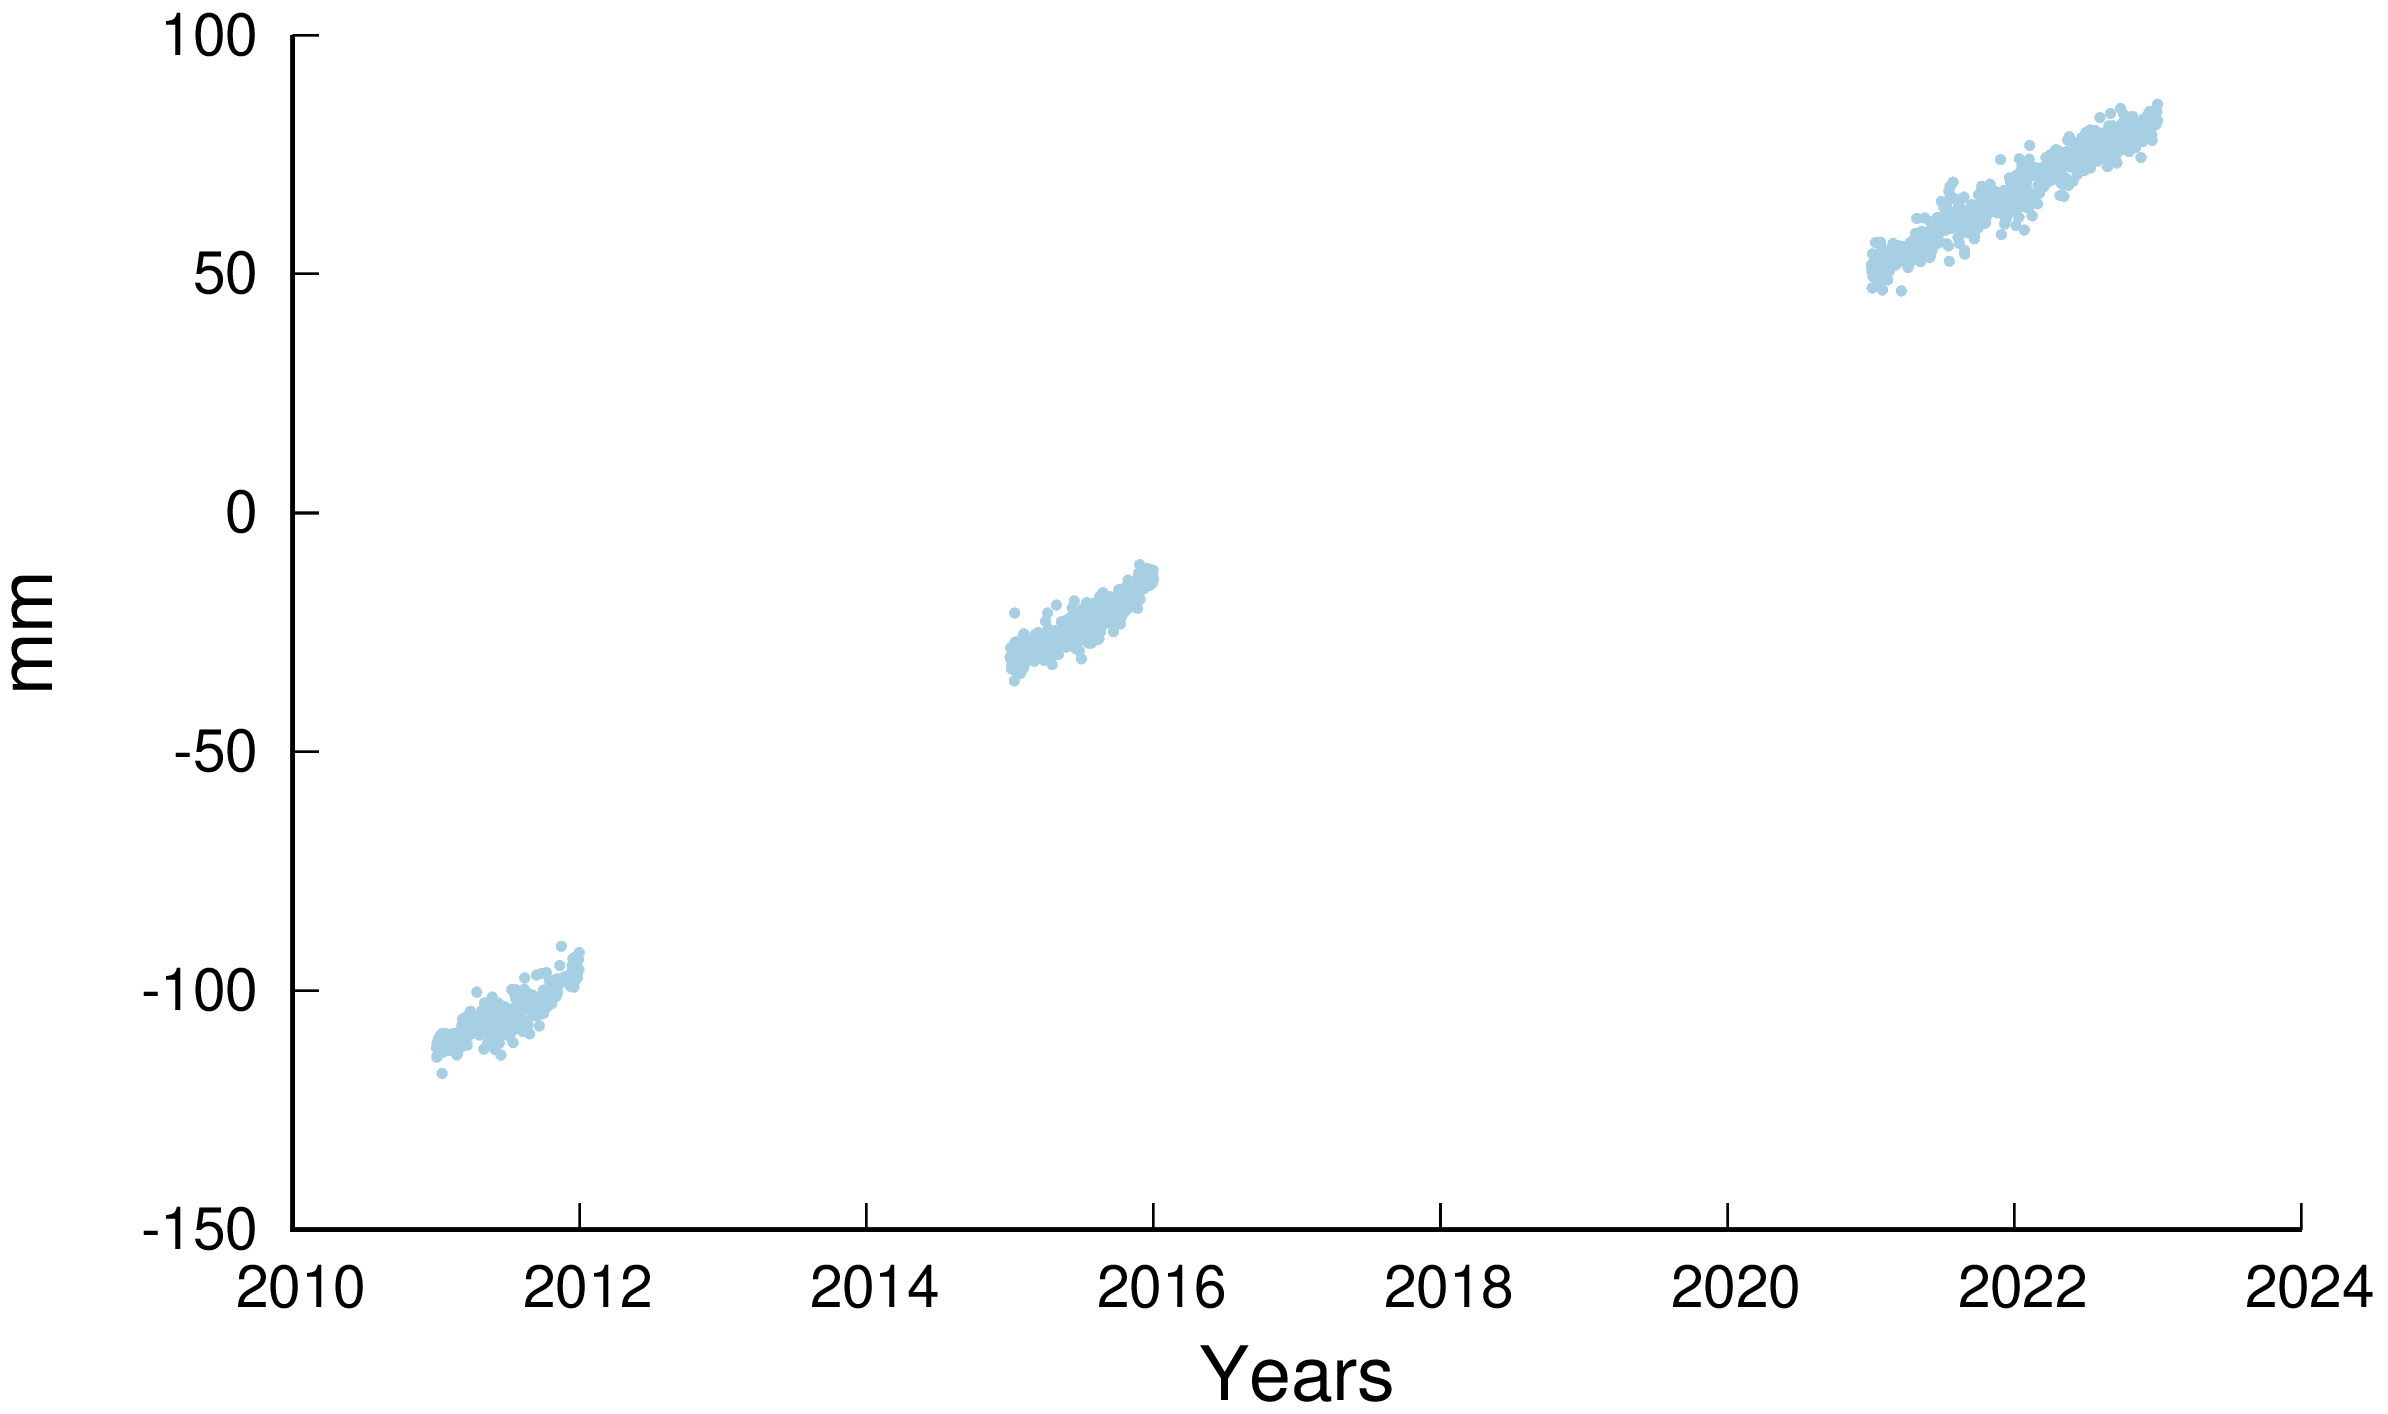
\includegraphics[width=.75\textwidth]{040a_1_data_nomodel.png}\\
         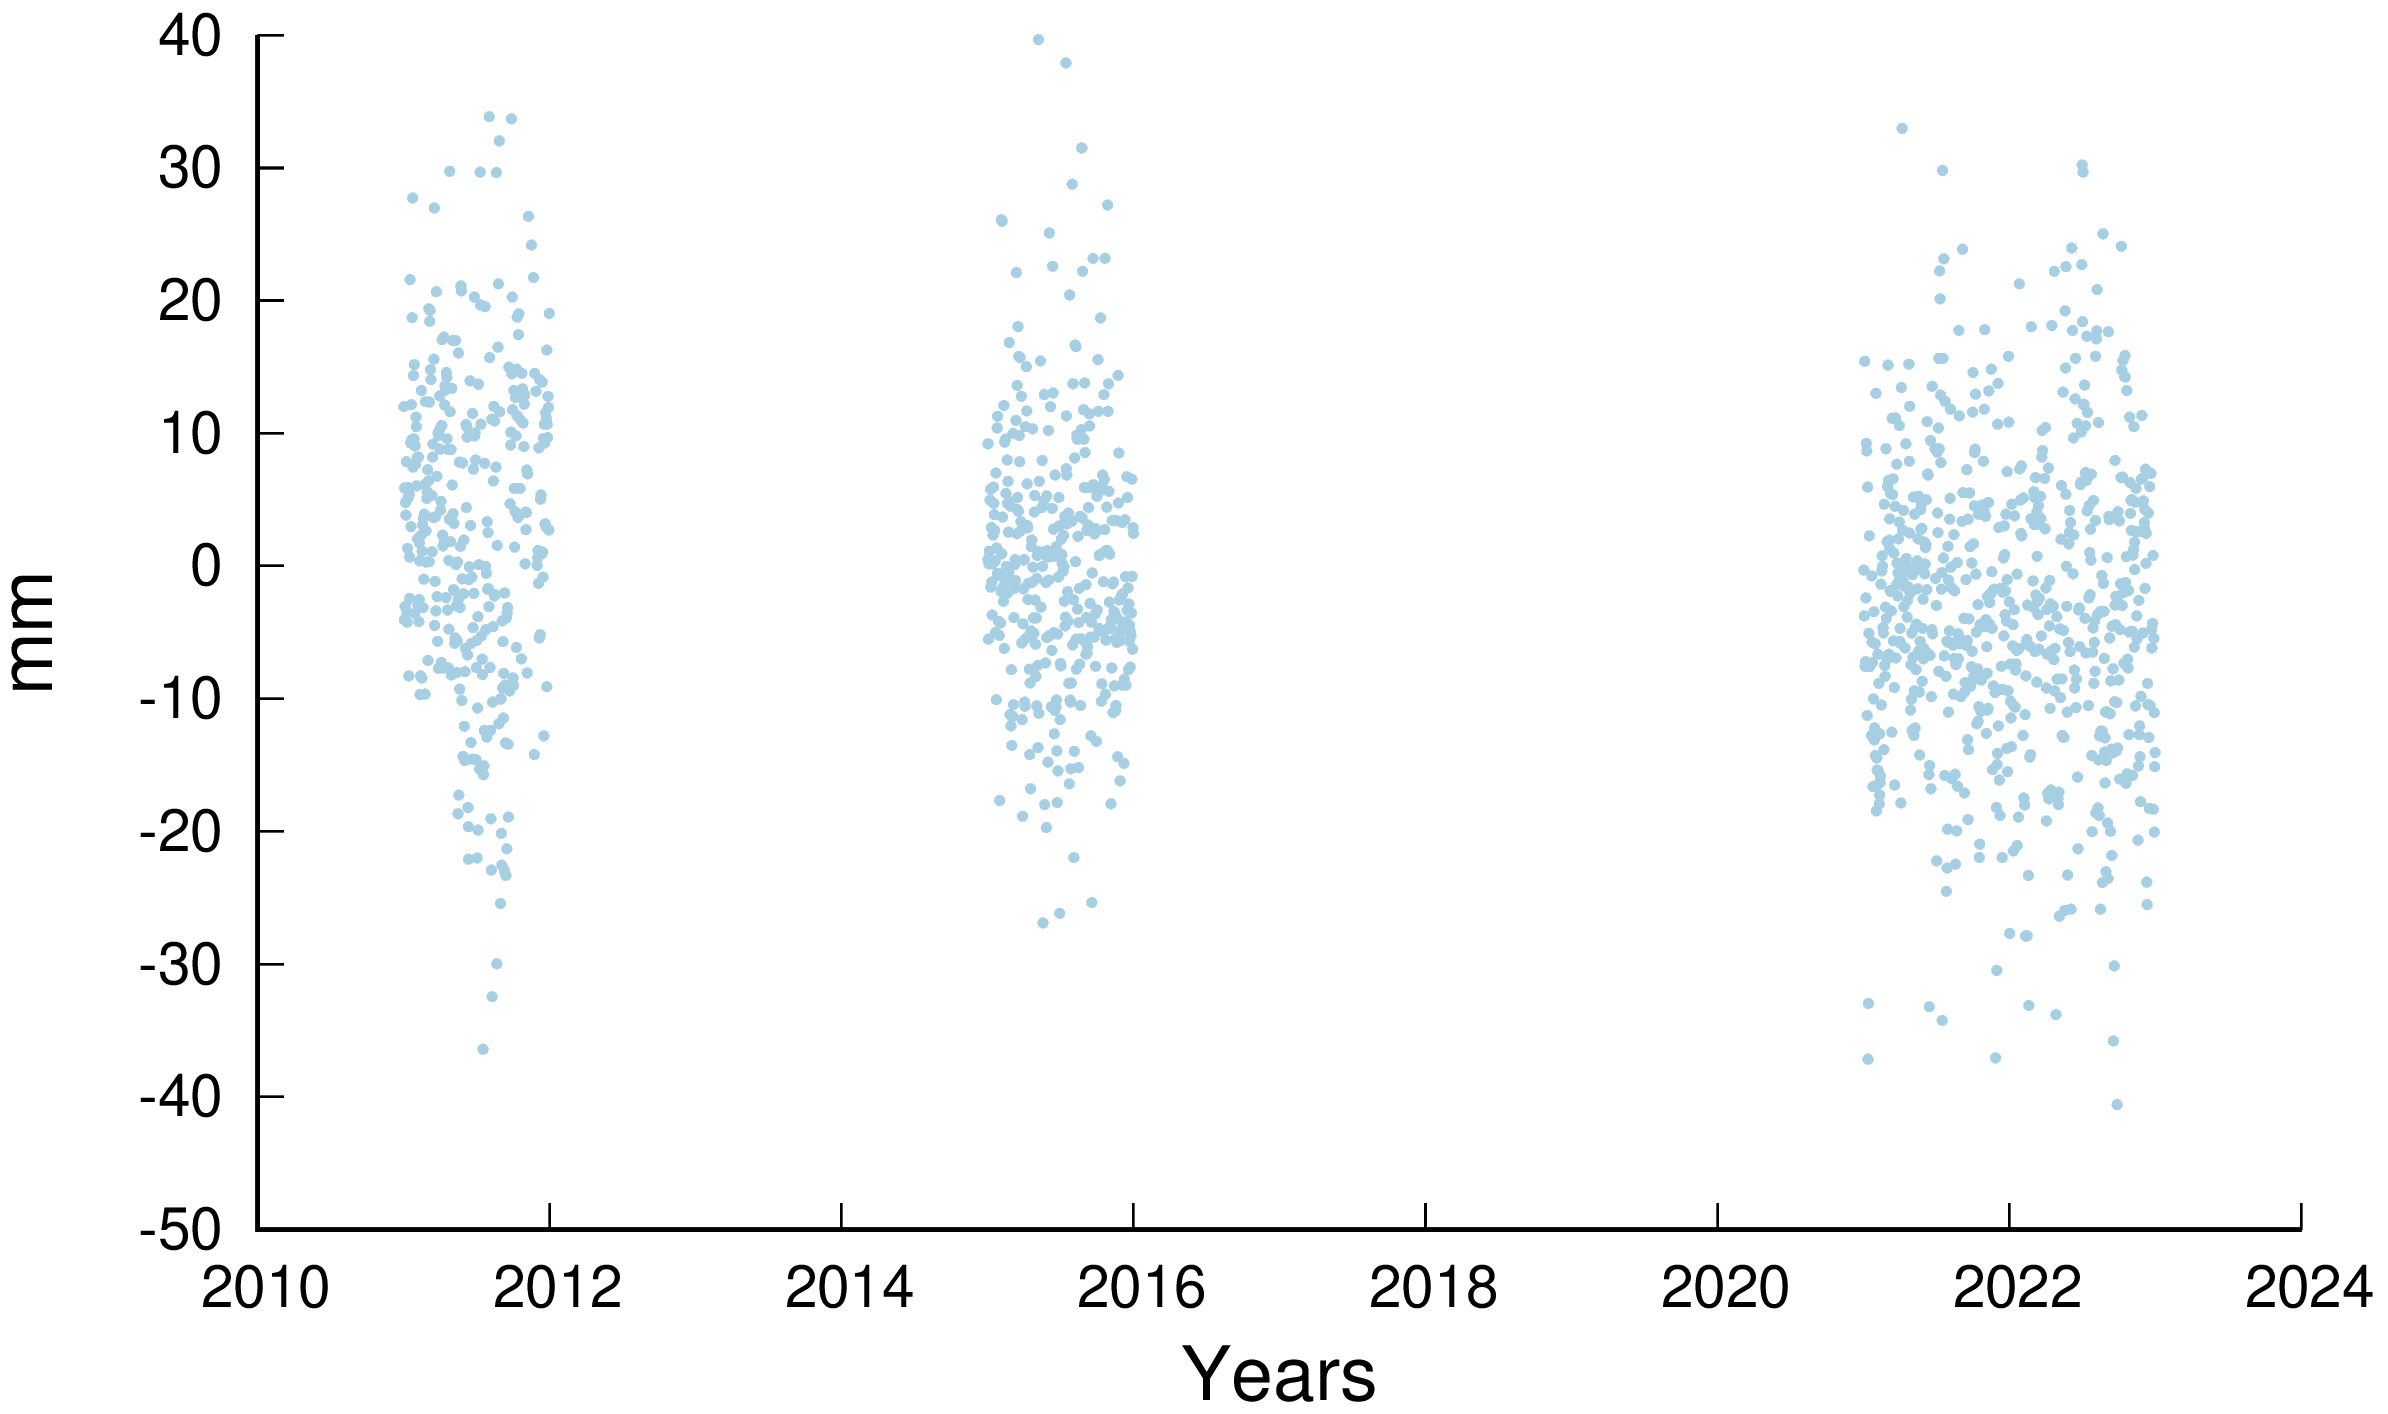
\includegraphics[width=.75\textwidth]{040a_2_data_nomodel.png}
       \end{center} 
    \end{column}
    \begin{column}{.33\textwidth}
      \begin{center}
      Station:\textbf{057A}\\
         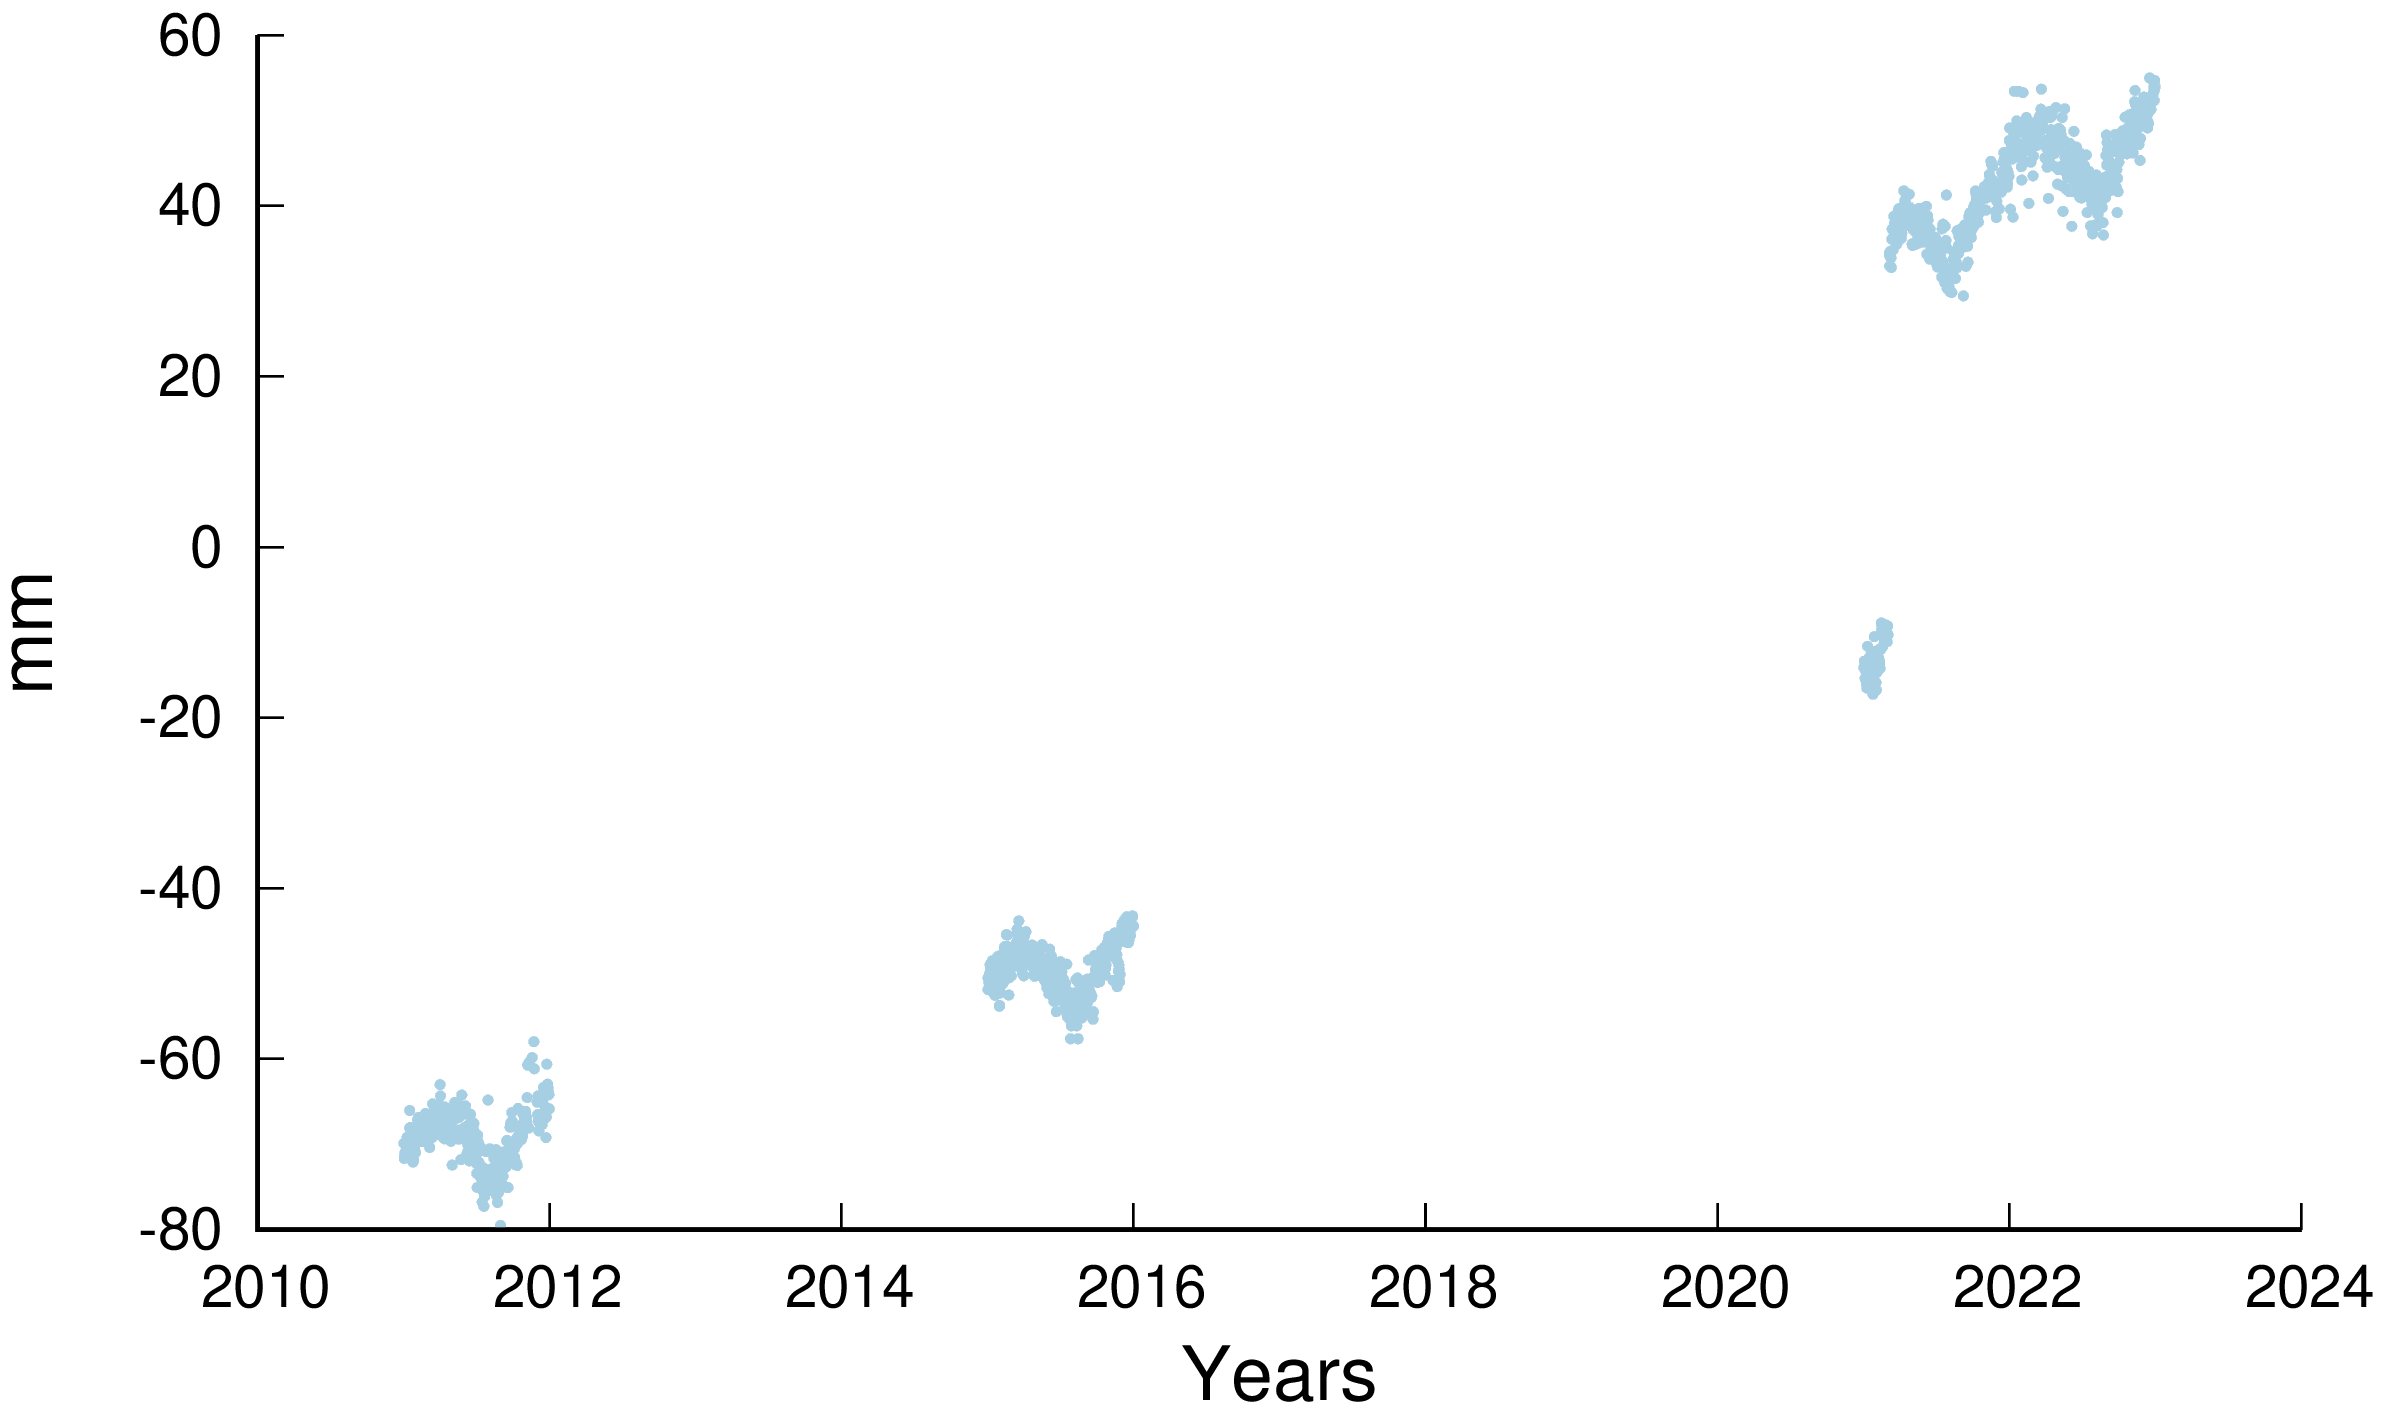
\includegraphics[width=.75\textwidth]{057a_0_data_nomodel.png}\\
         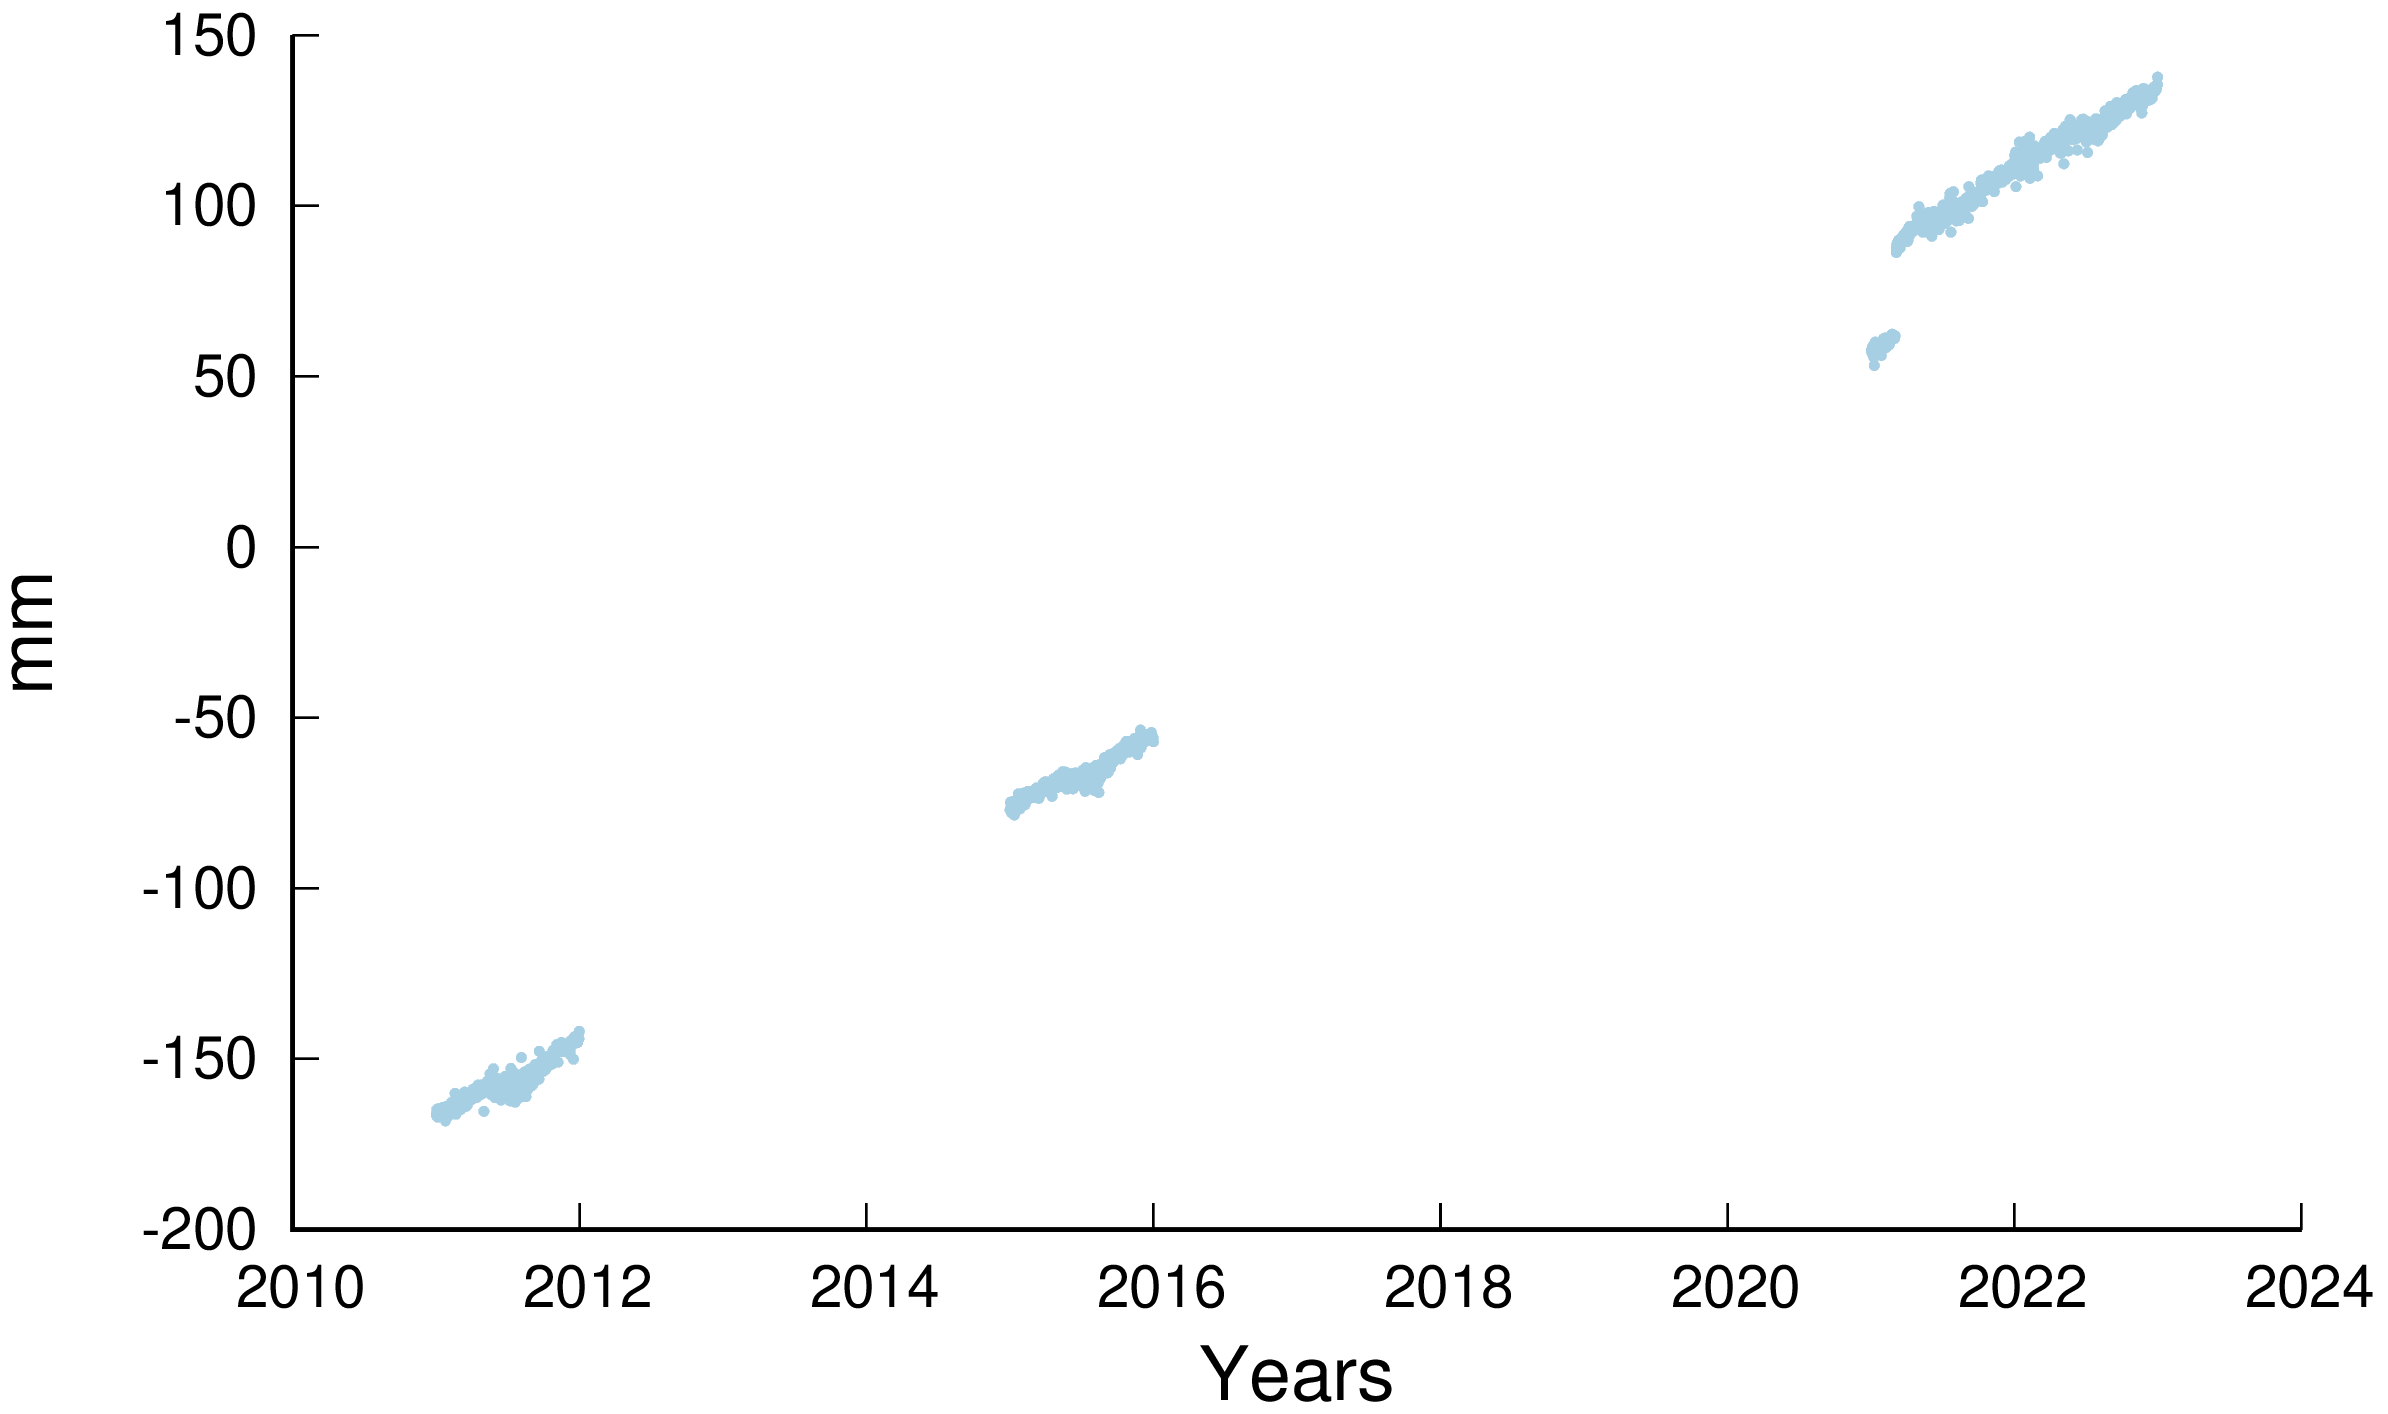
\includegraphics[width=.75\textwidth]{057a_1_data_nomodel.png}\\
         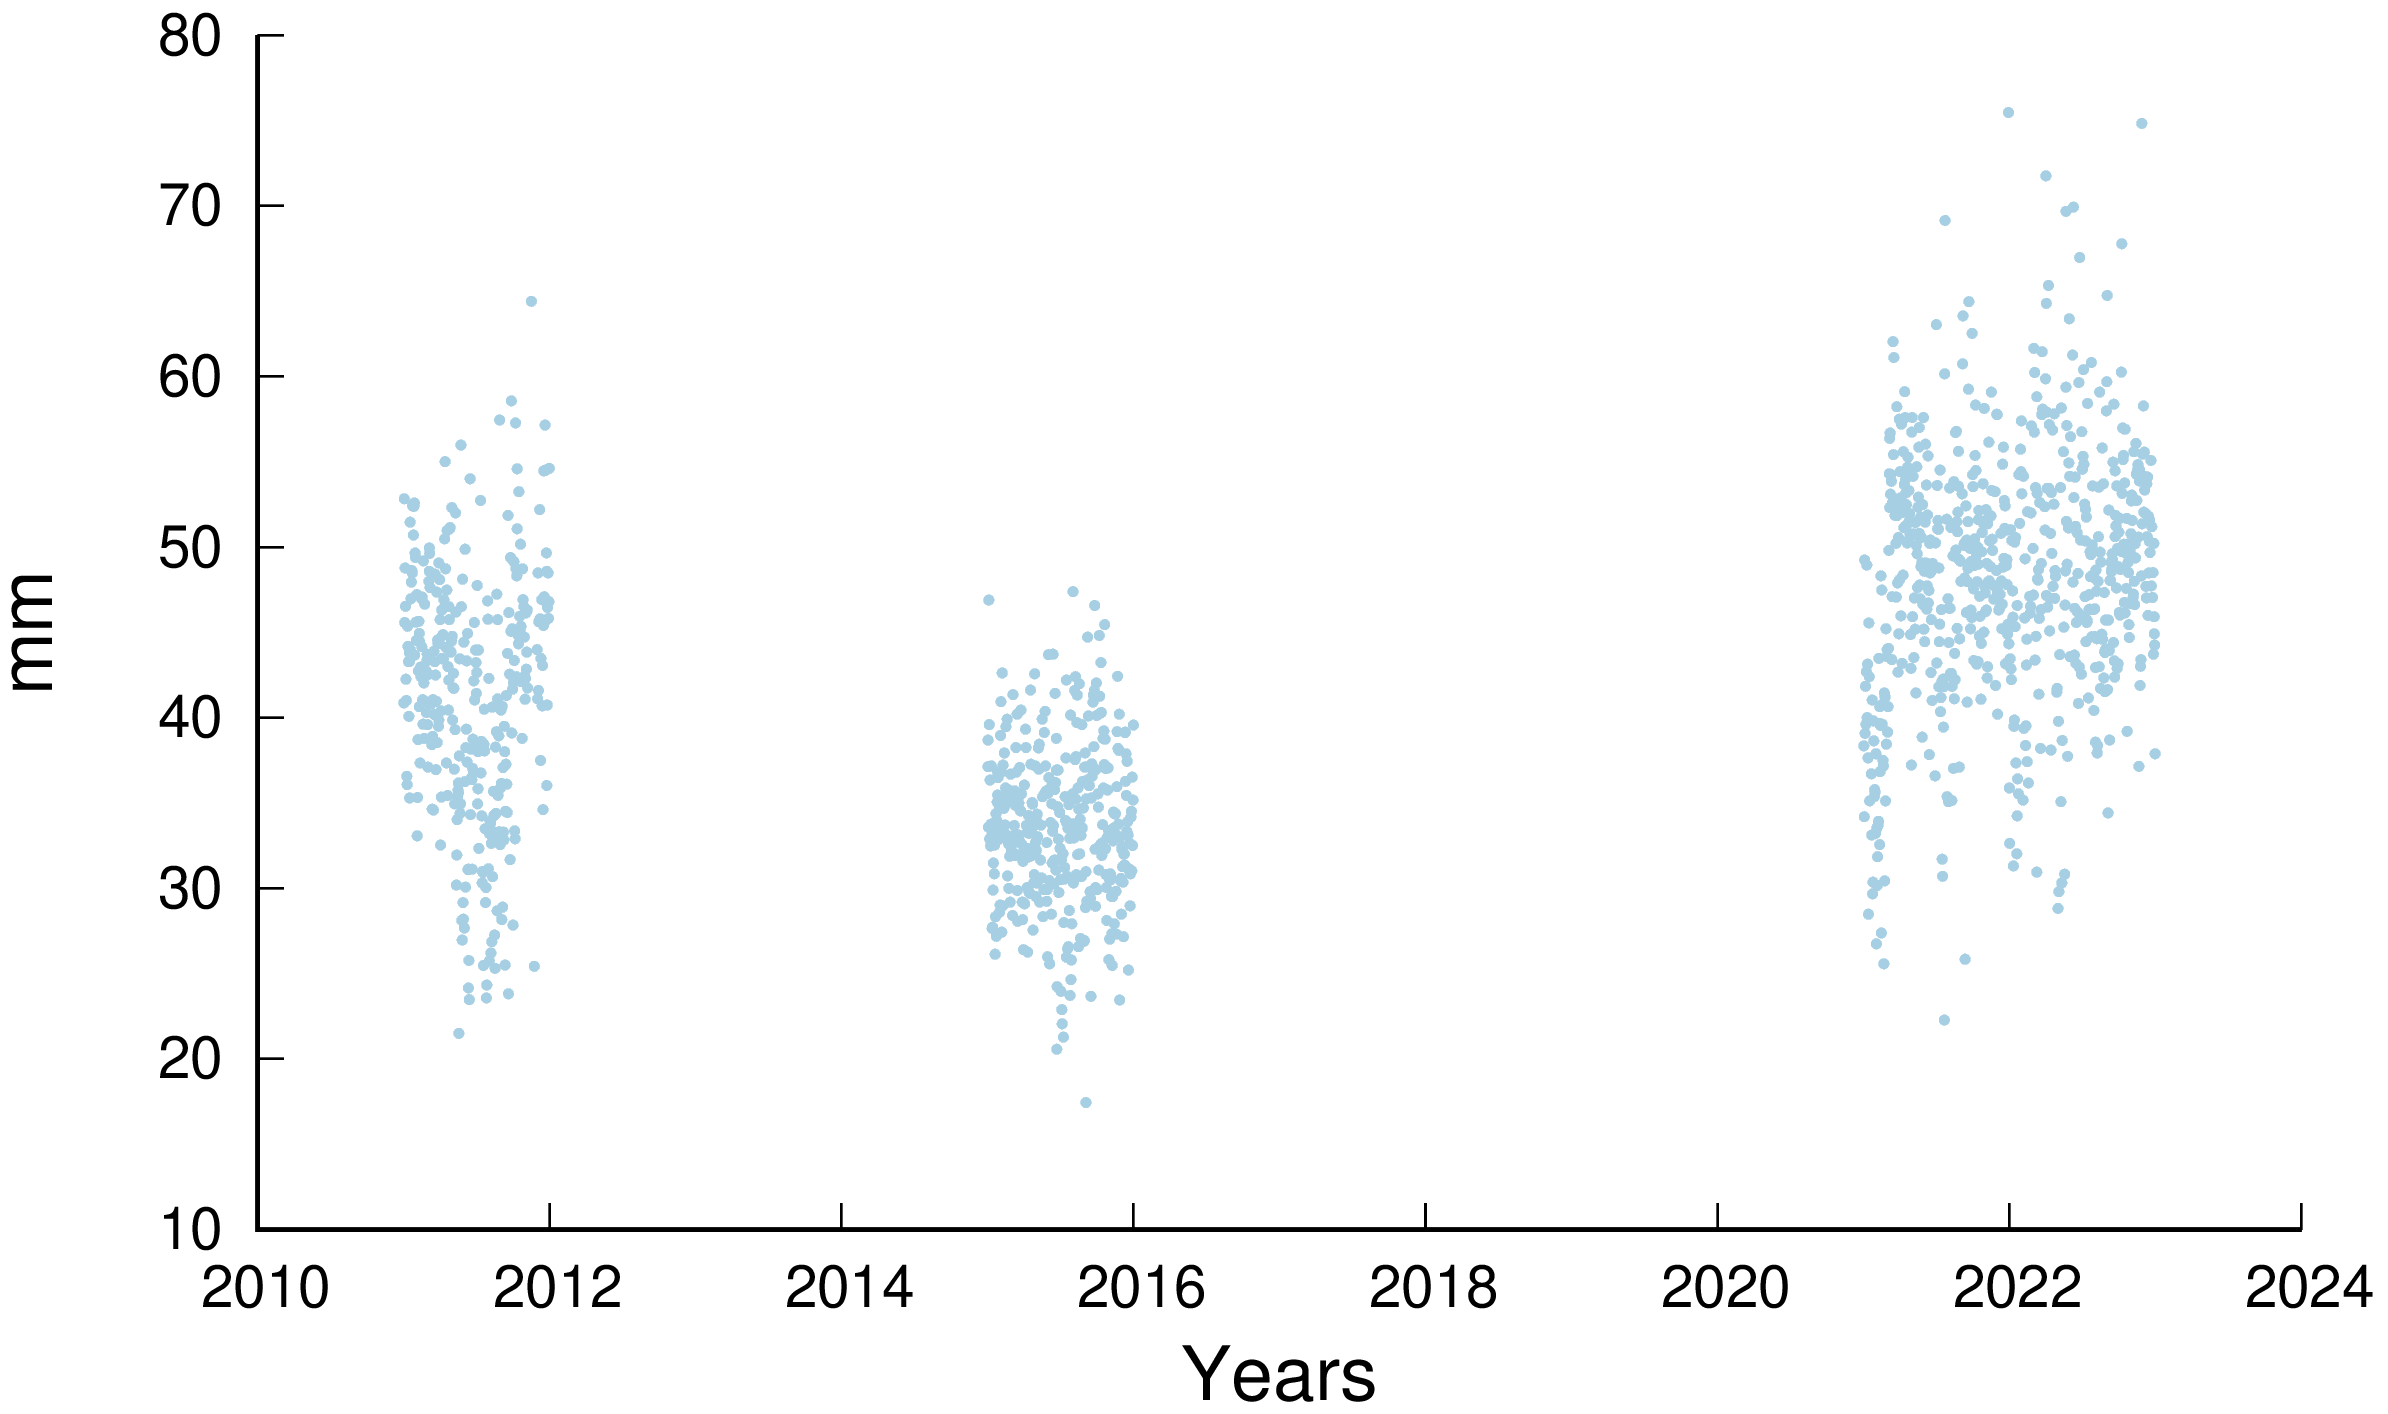
\includegraphics[width=.75\textwidth]{057a_2_data_nomodel.png}
       \end{center} 
    \end{column}
    \begin{column}{.33\textwidth}
      \begin{center}
      Station:\textbf{098A}\\
         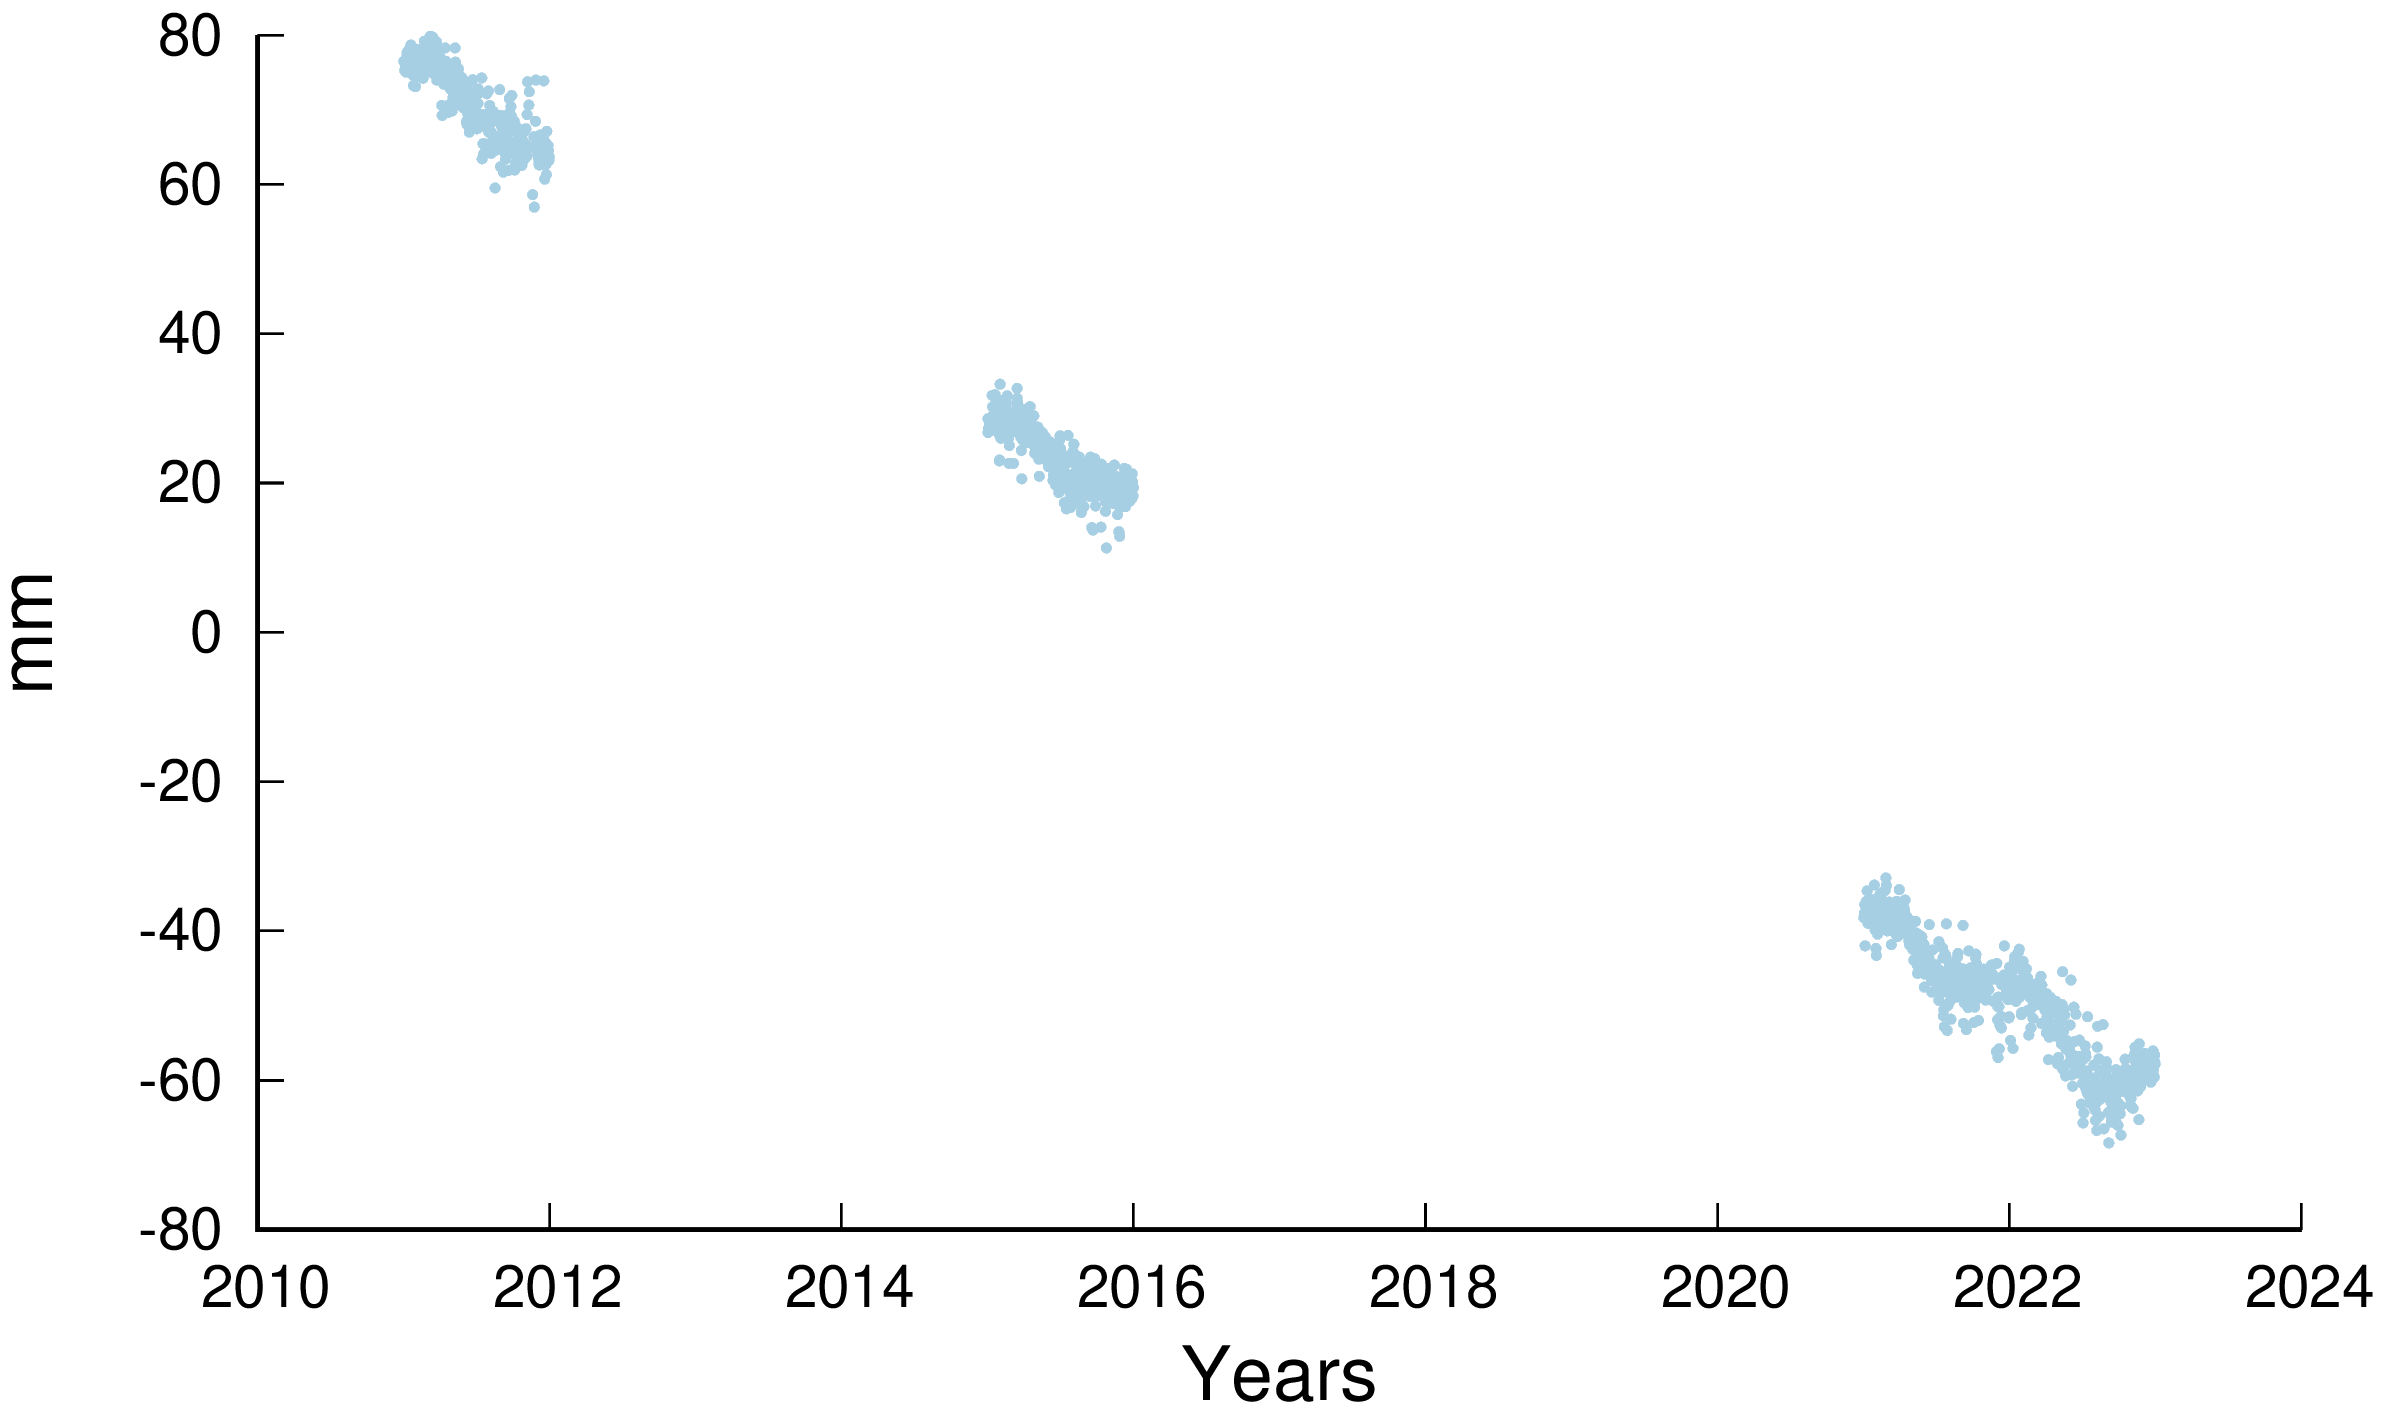
\includegraphics[width=.75\textwidth]{098a_0_data_nomodel.png}\\
         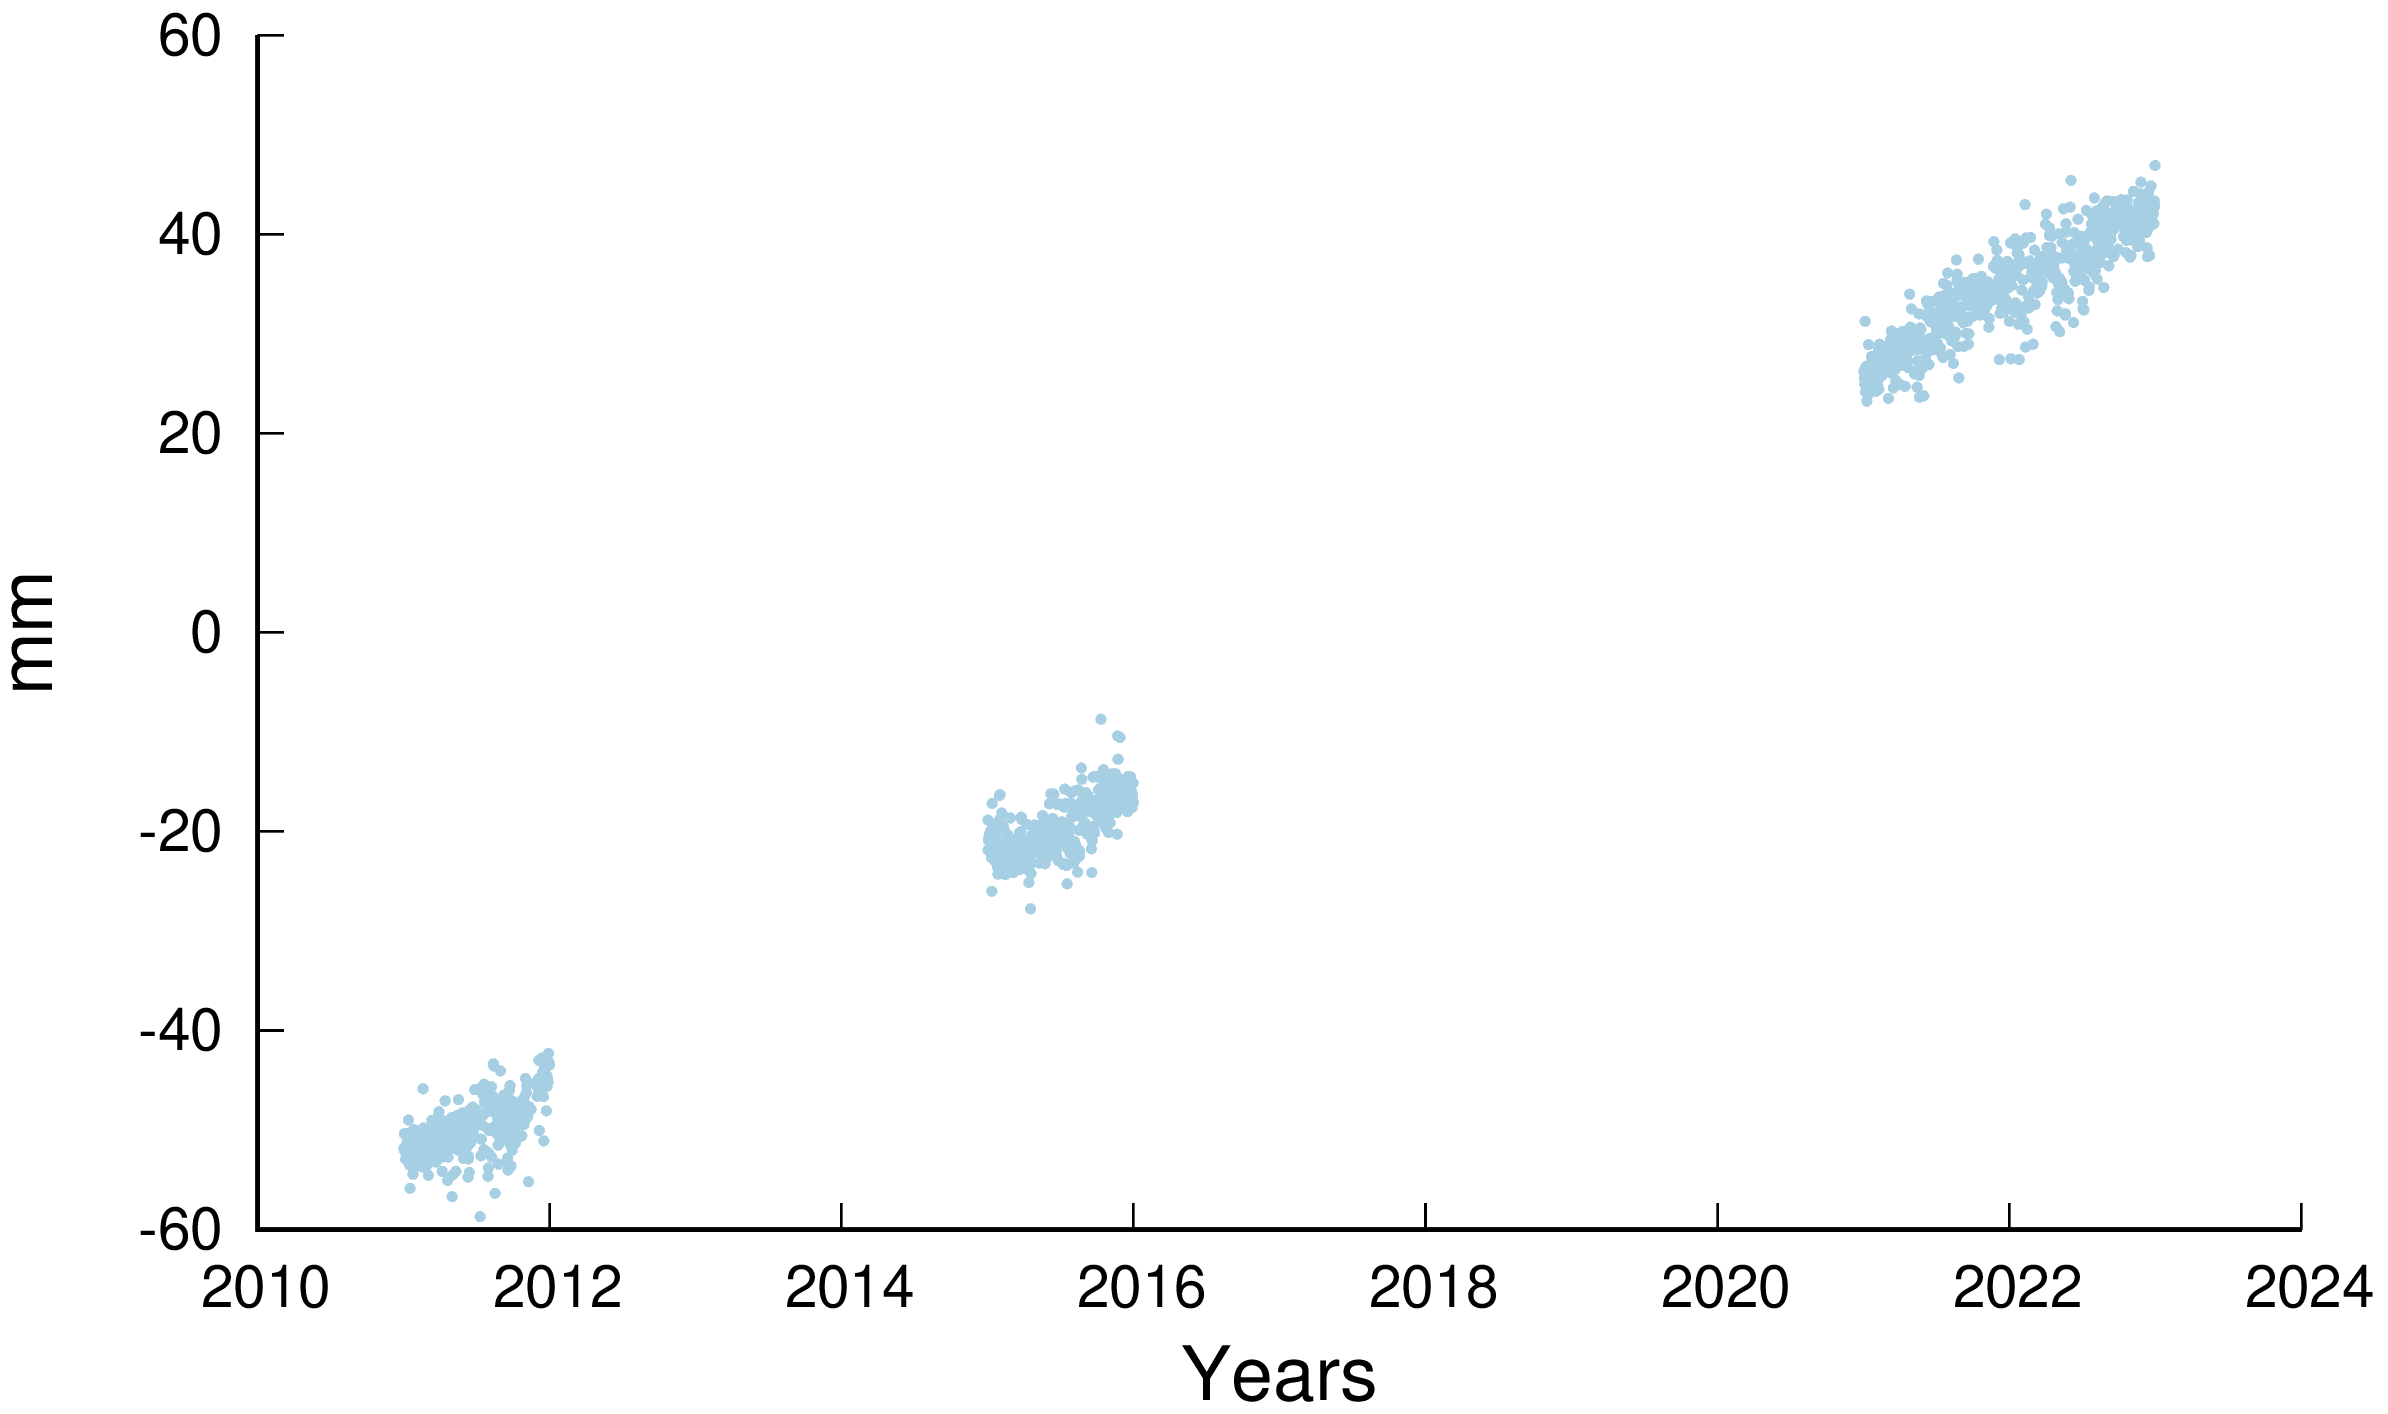
\includegraphics[width=.75\textwidth]{098a_1_data_nomodel.png}\\
         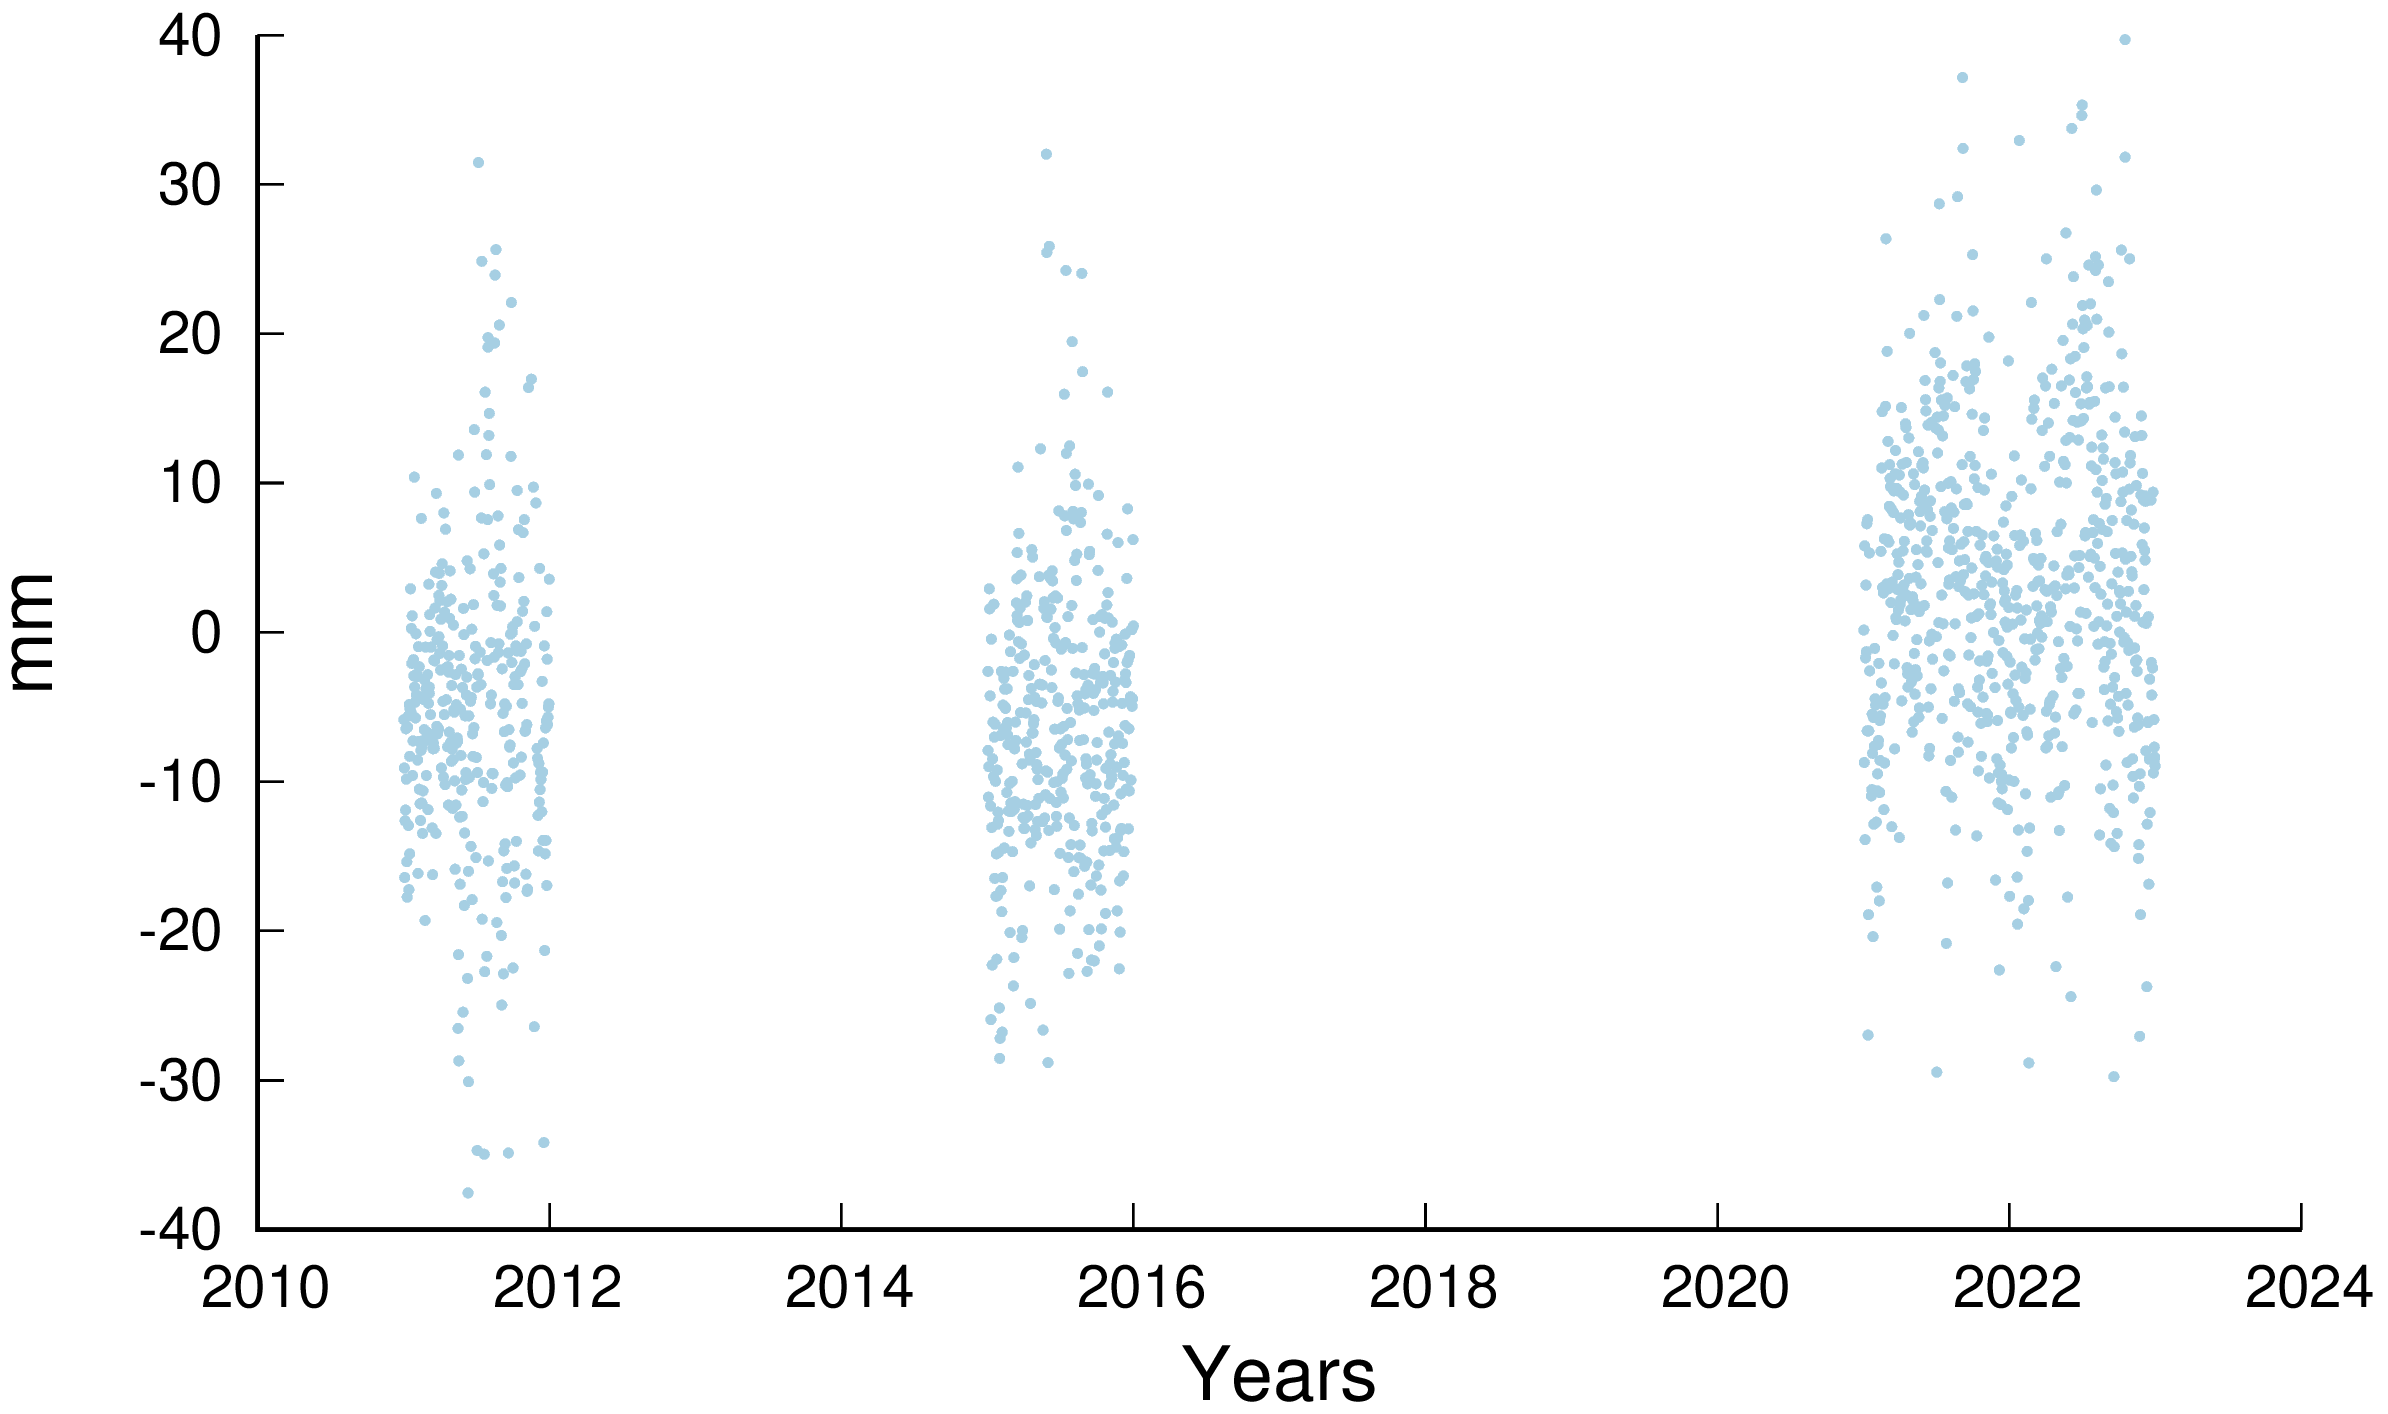
\includegraphics[width=.75\textwidth]{098a_2_data_nomodel.png}
       \end{center} 
      
    \end{column}
  \end{columns}
\end{frame}
\note{}

 % ------------------------------------------------------------------------------
\begin{frame}
  \frametitle{Συσχετισμός ασυνεχειών με σεισμούς}
  \framesubtitle{}
  \label{}
  \vskip-1cm
  \begin{columns}[T]
    \begin{column}{.33\textwidth}
      \begin{table}[H]{\small
      \begin{center}
      \begin{tabular*}{.97\linewidth}{@{\extracolsep{\fill}} c c c c}
        \toprule
         date & Δn & Δe & Δu\\
              & \multicolumn{3}{c}{(mm)}\\
        \midrule
        \multicolumn{4}{l}{Station: 040A}\\
        26.01.2014 & -43.1 & 25.2 & 2.2 \\
        17.11.2015 & -10.8 & 1.7 & 3.1\\
        \midrule
        \multicolumn{4}{l}{Station: 057A}\\
        03.03.2021 & 47.9 & 27.6 & 14.0\\
        \bottomrule
      \end{tabular*}
      \end{center}}
      \end{table}
    \end{column}
    \begin{column}{.33\textwidth}
      \begin{center}
      Station:\textbf{040A}\\
         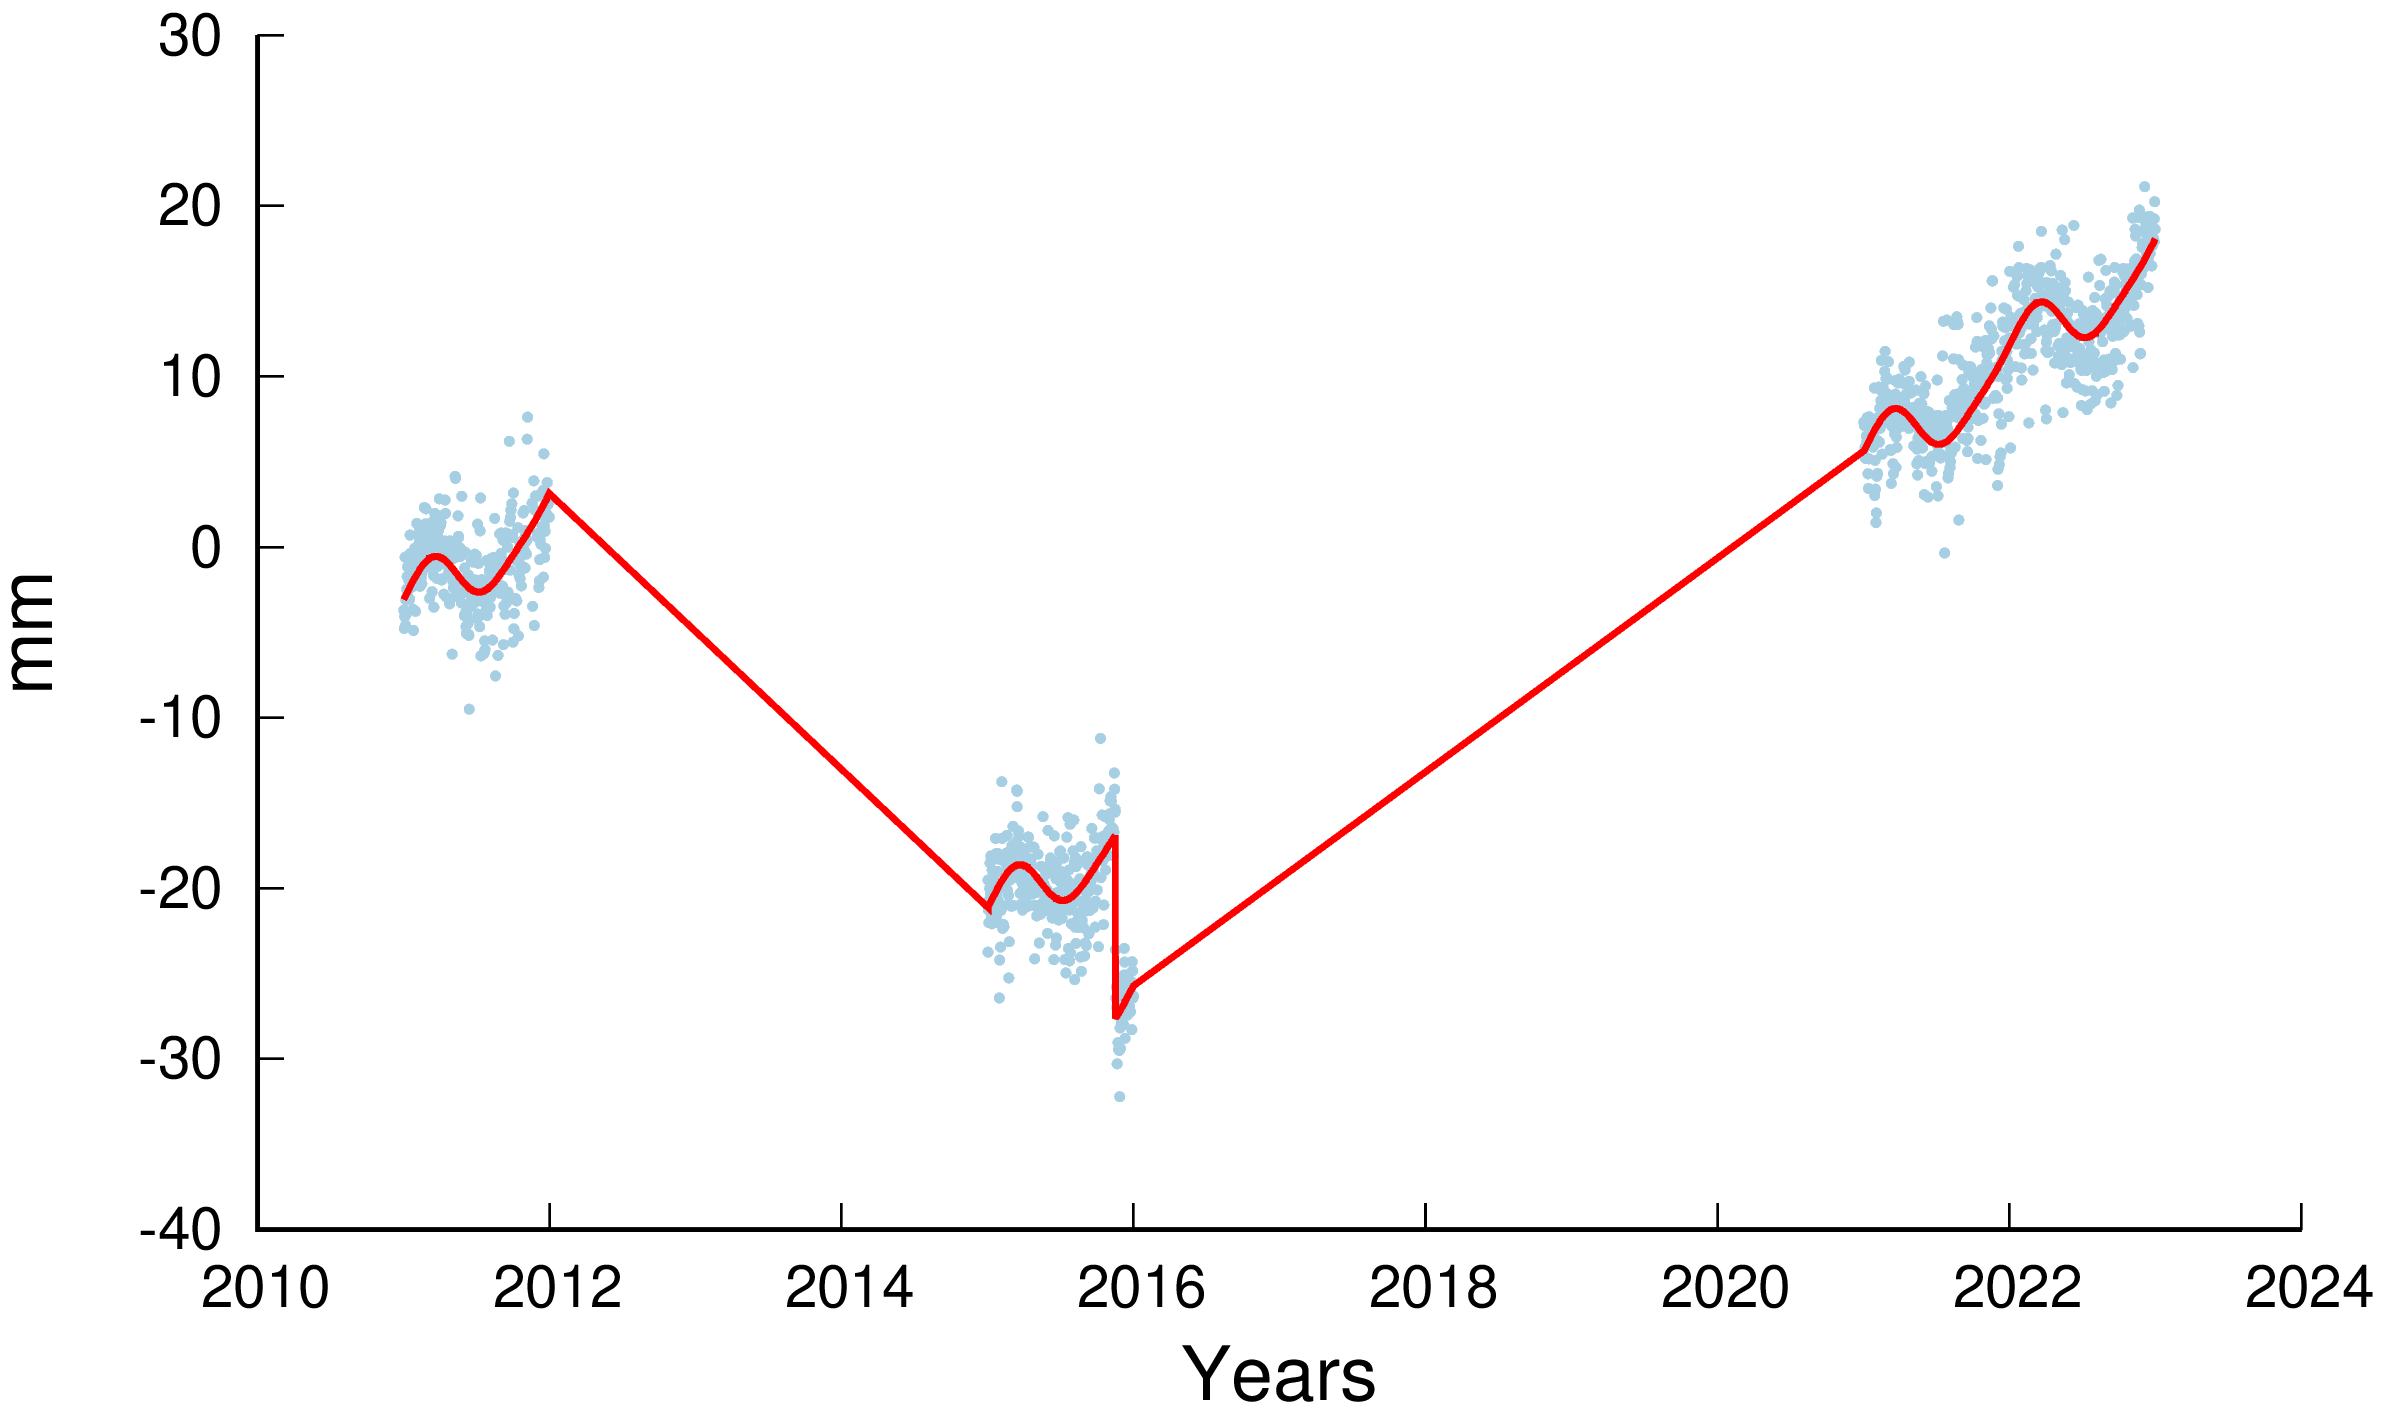
\includegraphics[width=.75\textwidth]{040a_0_data.png}\\
         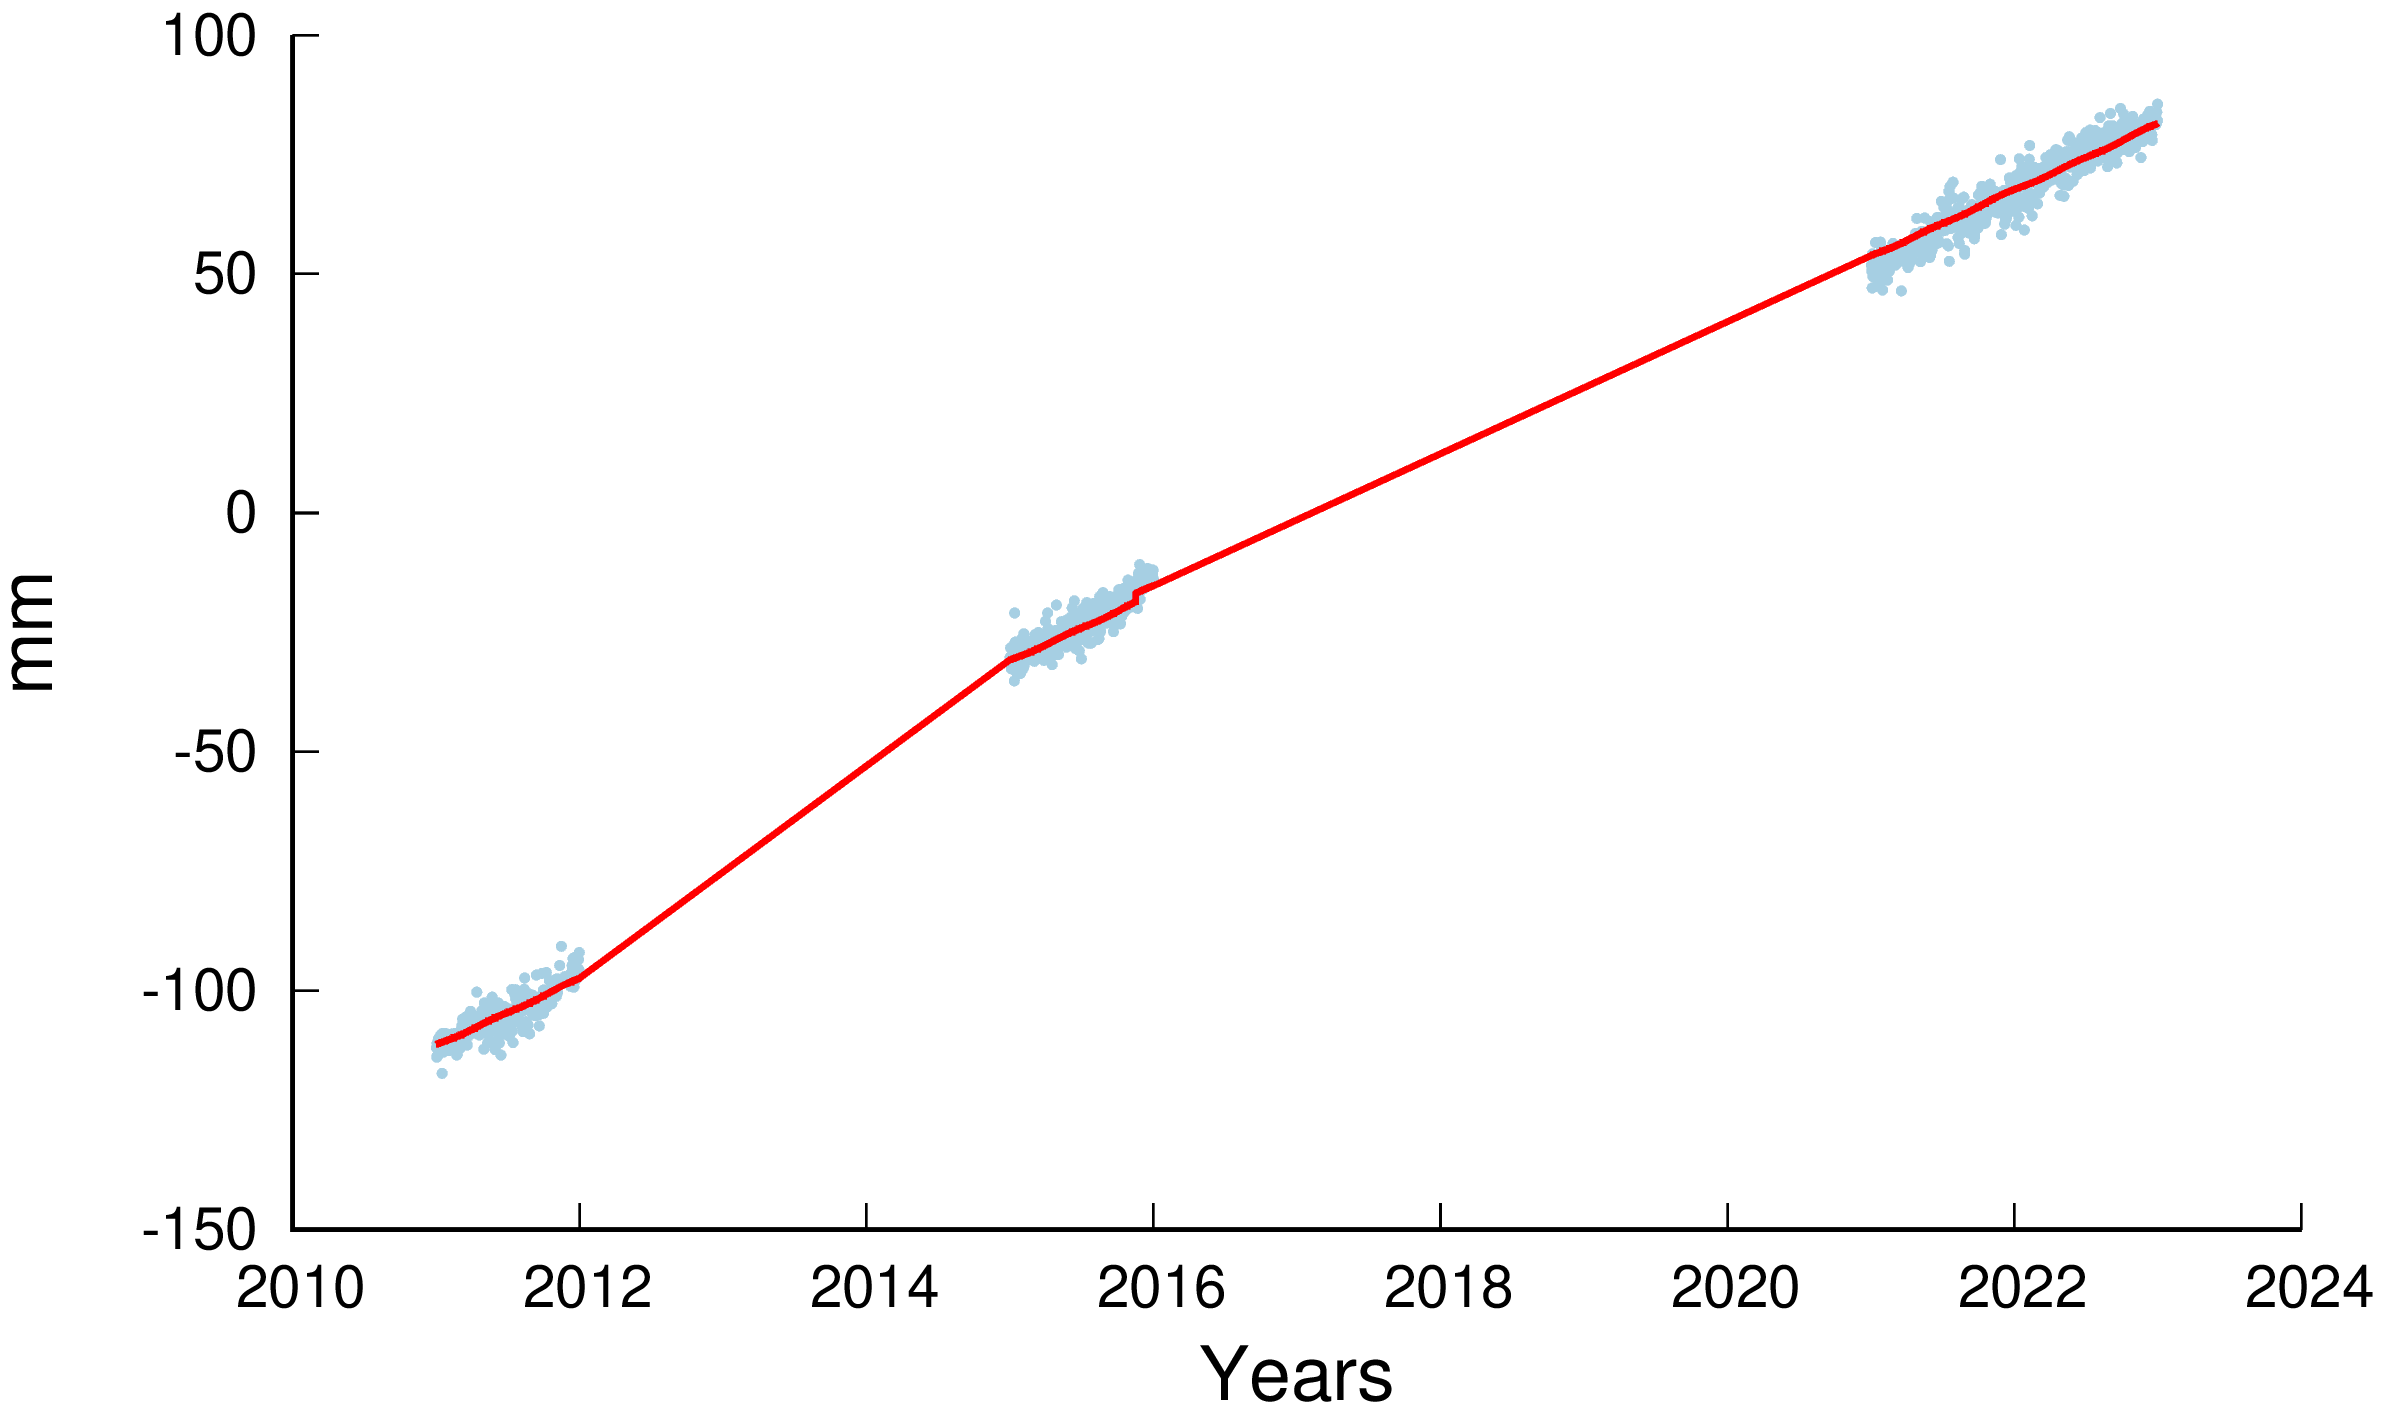
\includegraphics[width=.75\textwidth]{040a_1_data.png}\\
         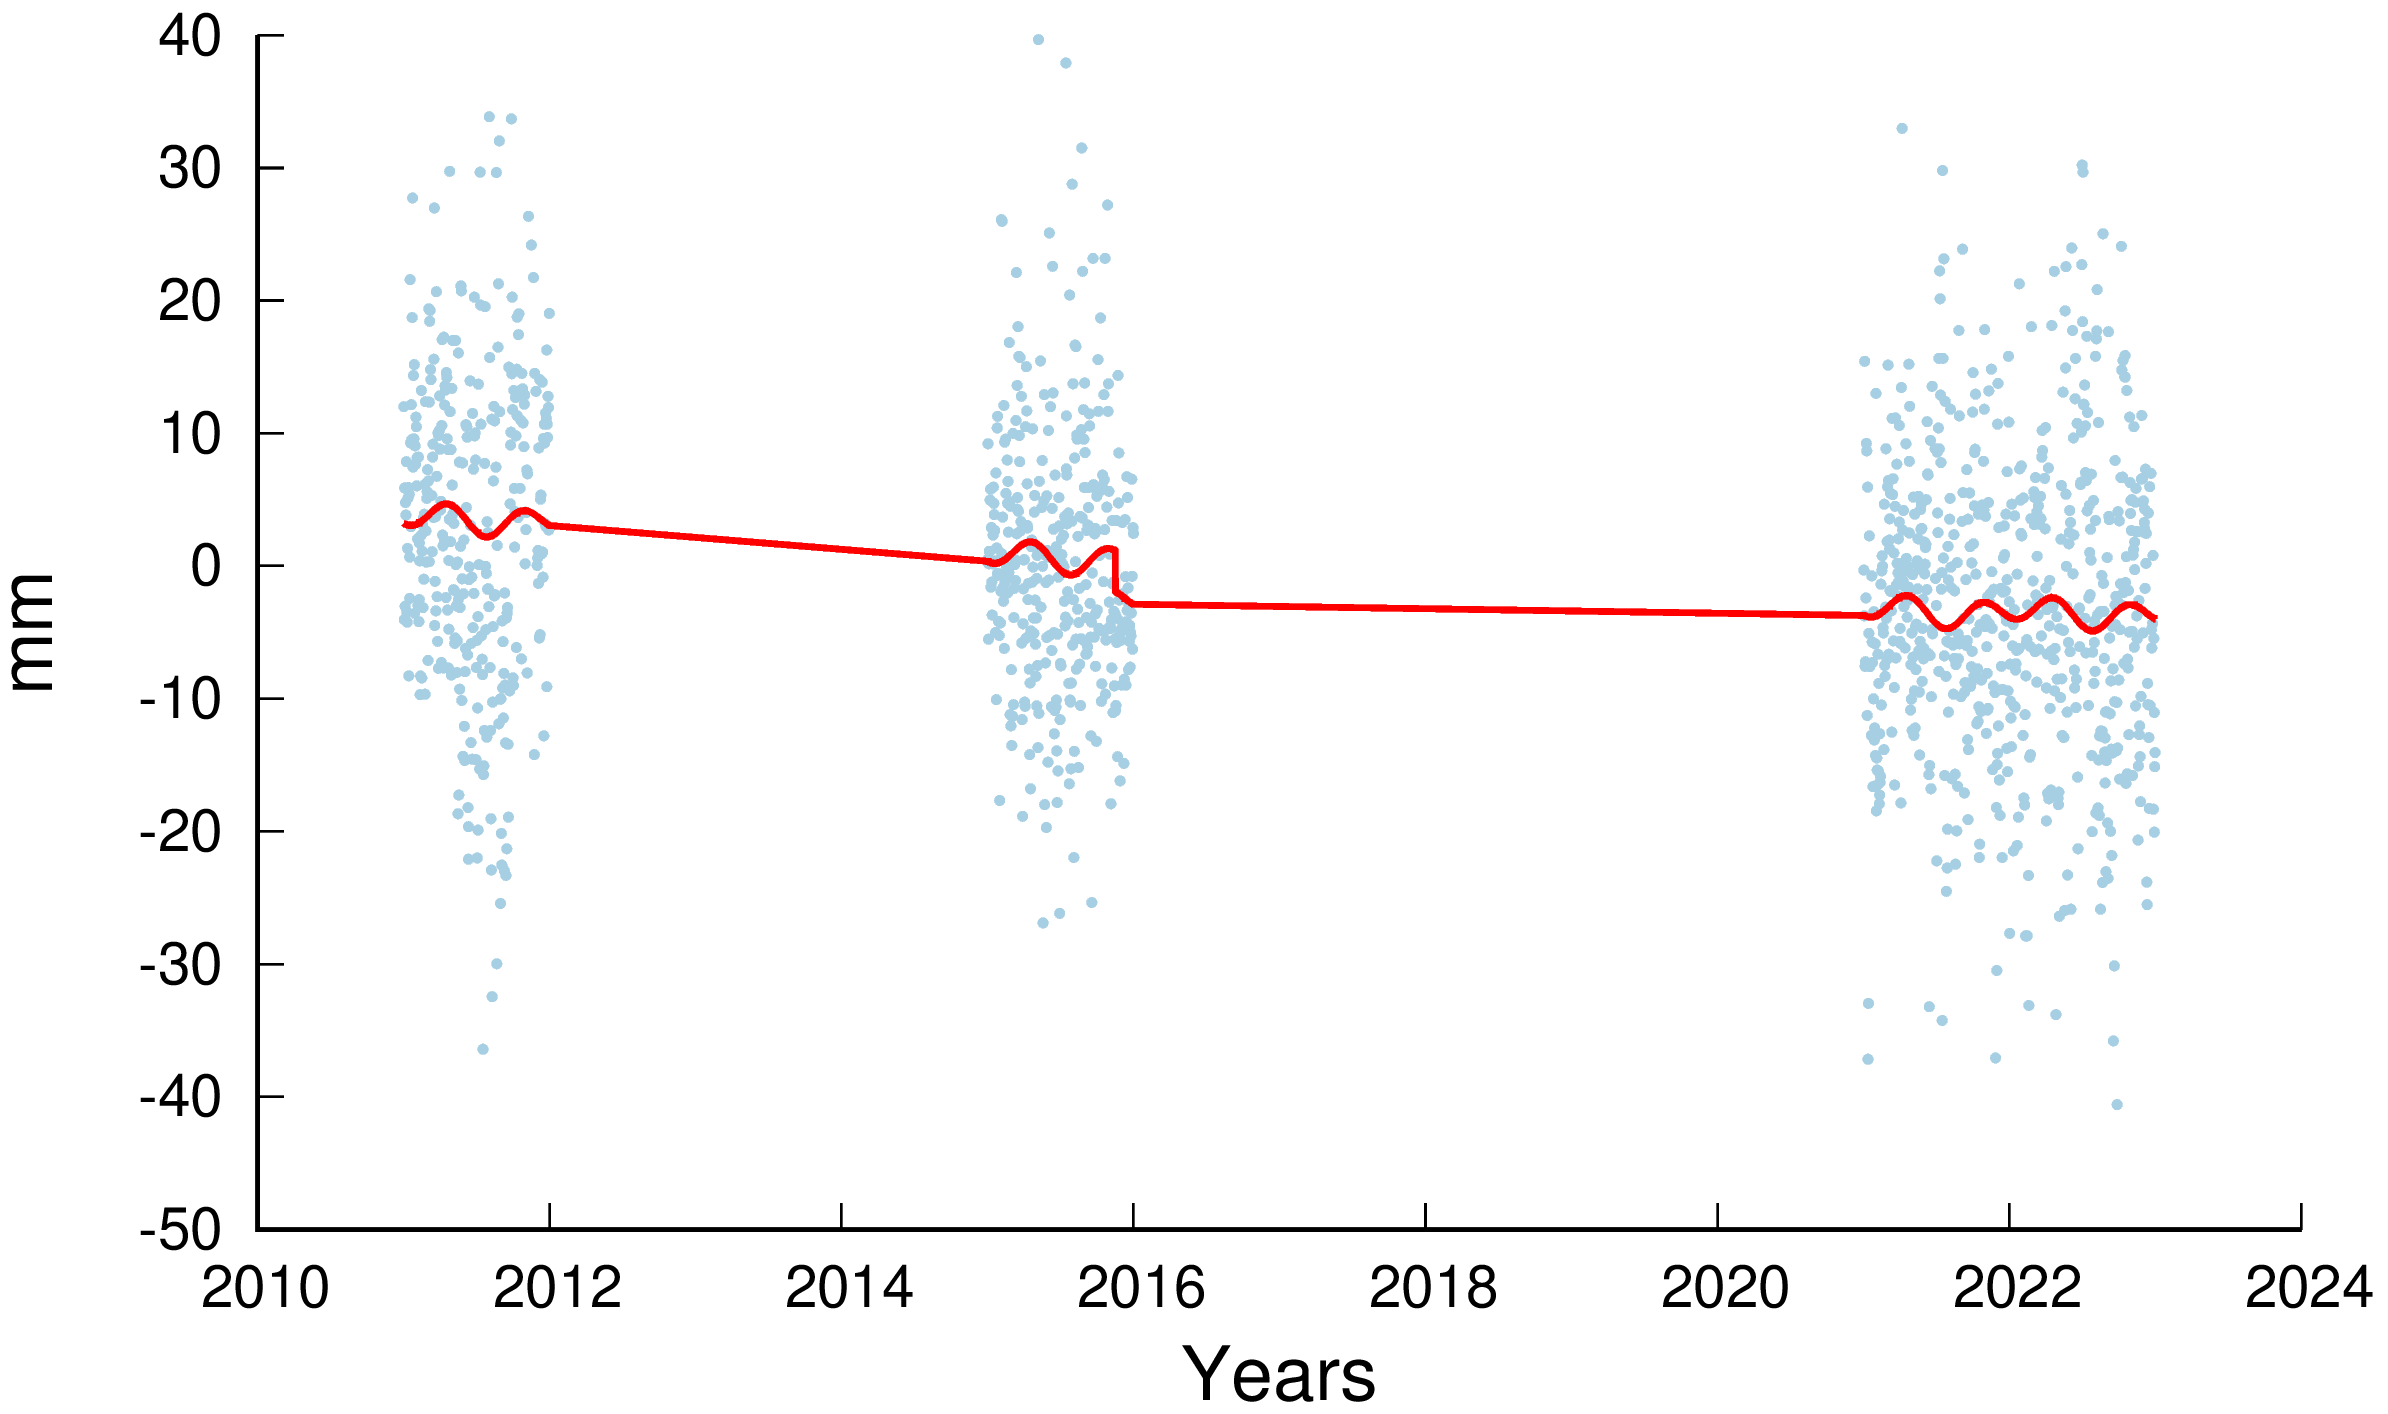
\includegraphics[width=.75\textwidth]{040a_2_data.png}
       \end{center} 
    \end{column}
    \begin{column}{.33\textwidth}
      \begin{center}
      Station:\textbf{057A}\\
         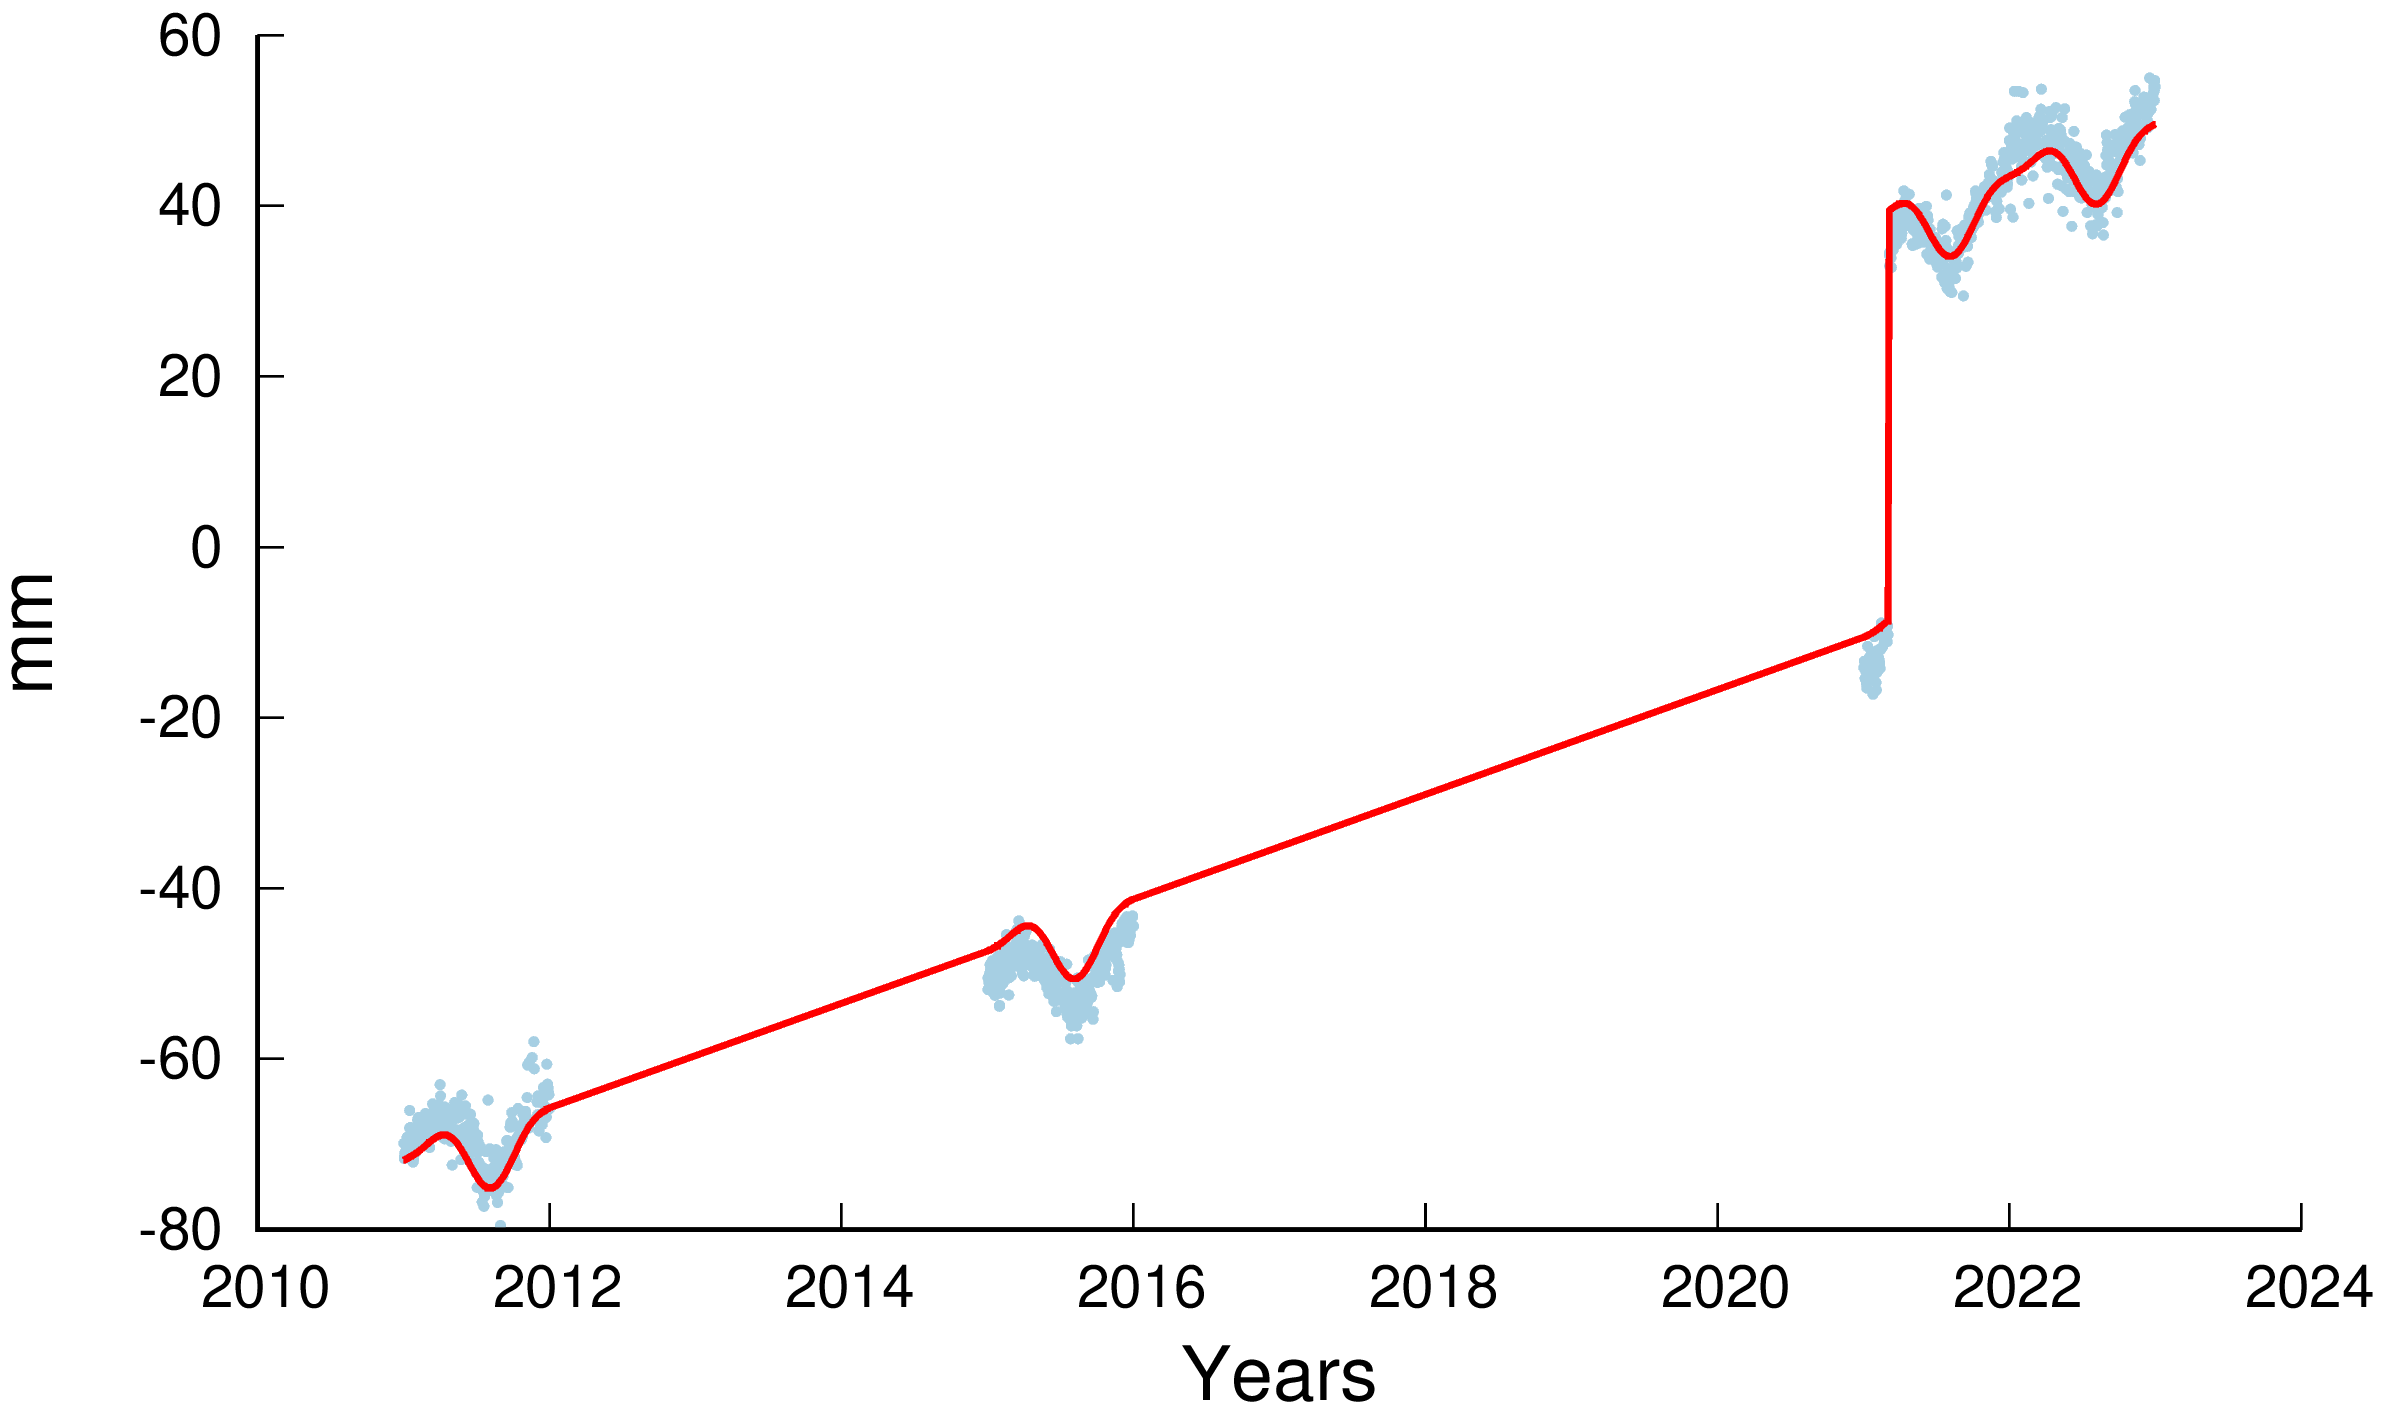
\includegraphics[width=.75\textwidth]{057a_0_data.png}\\
         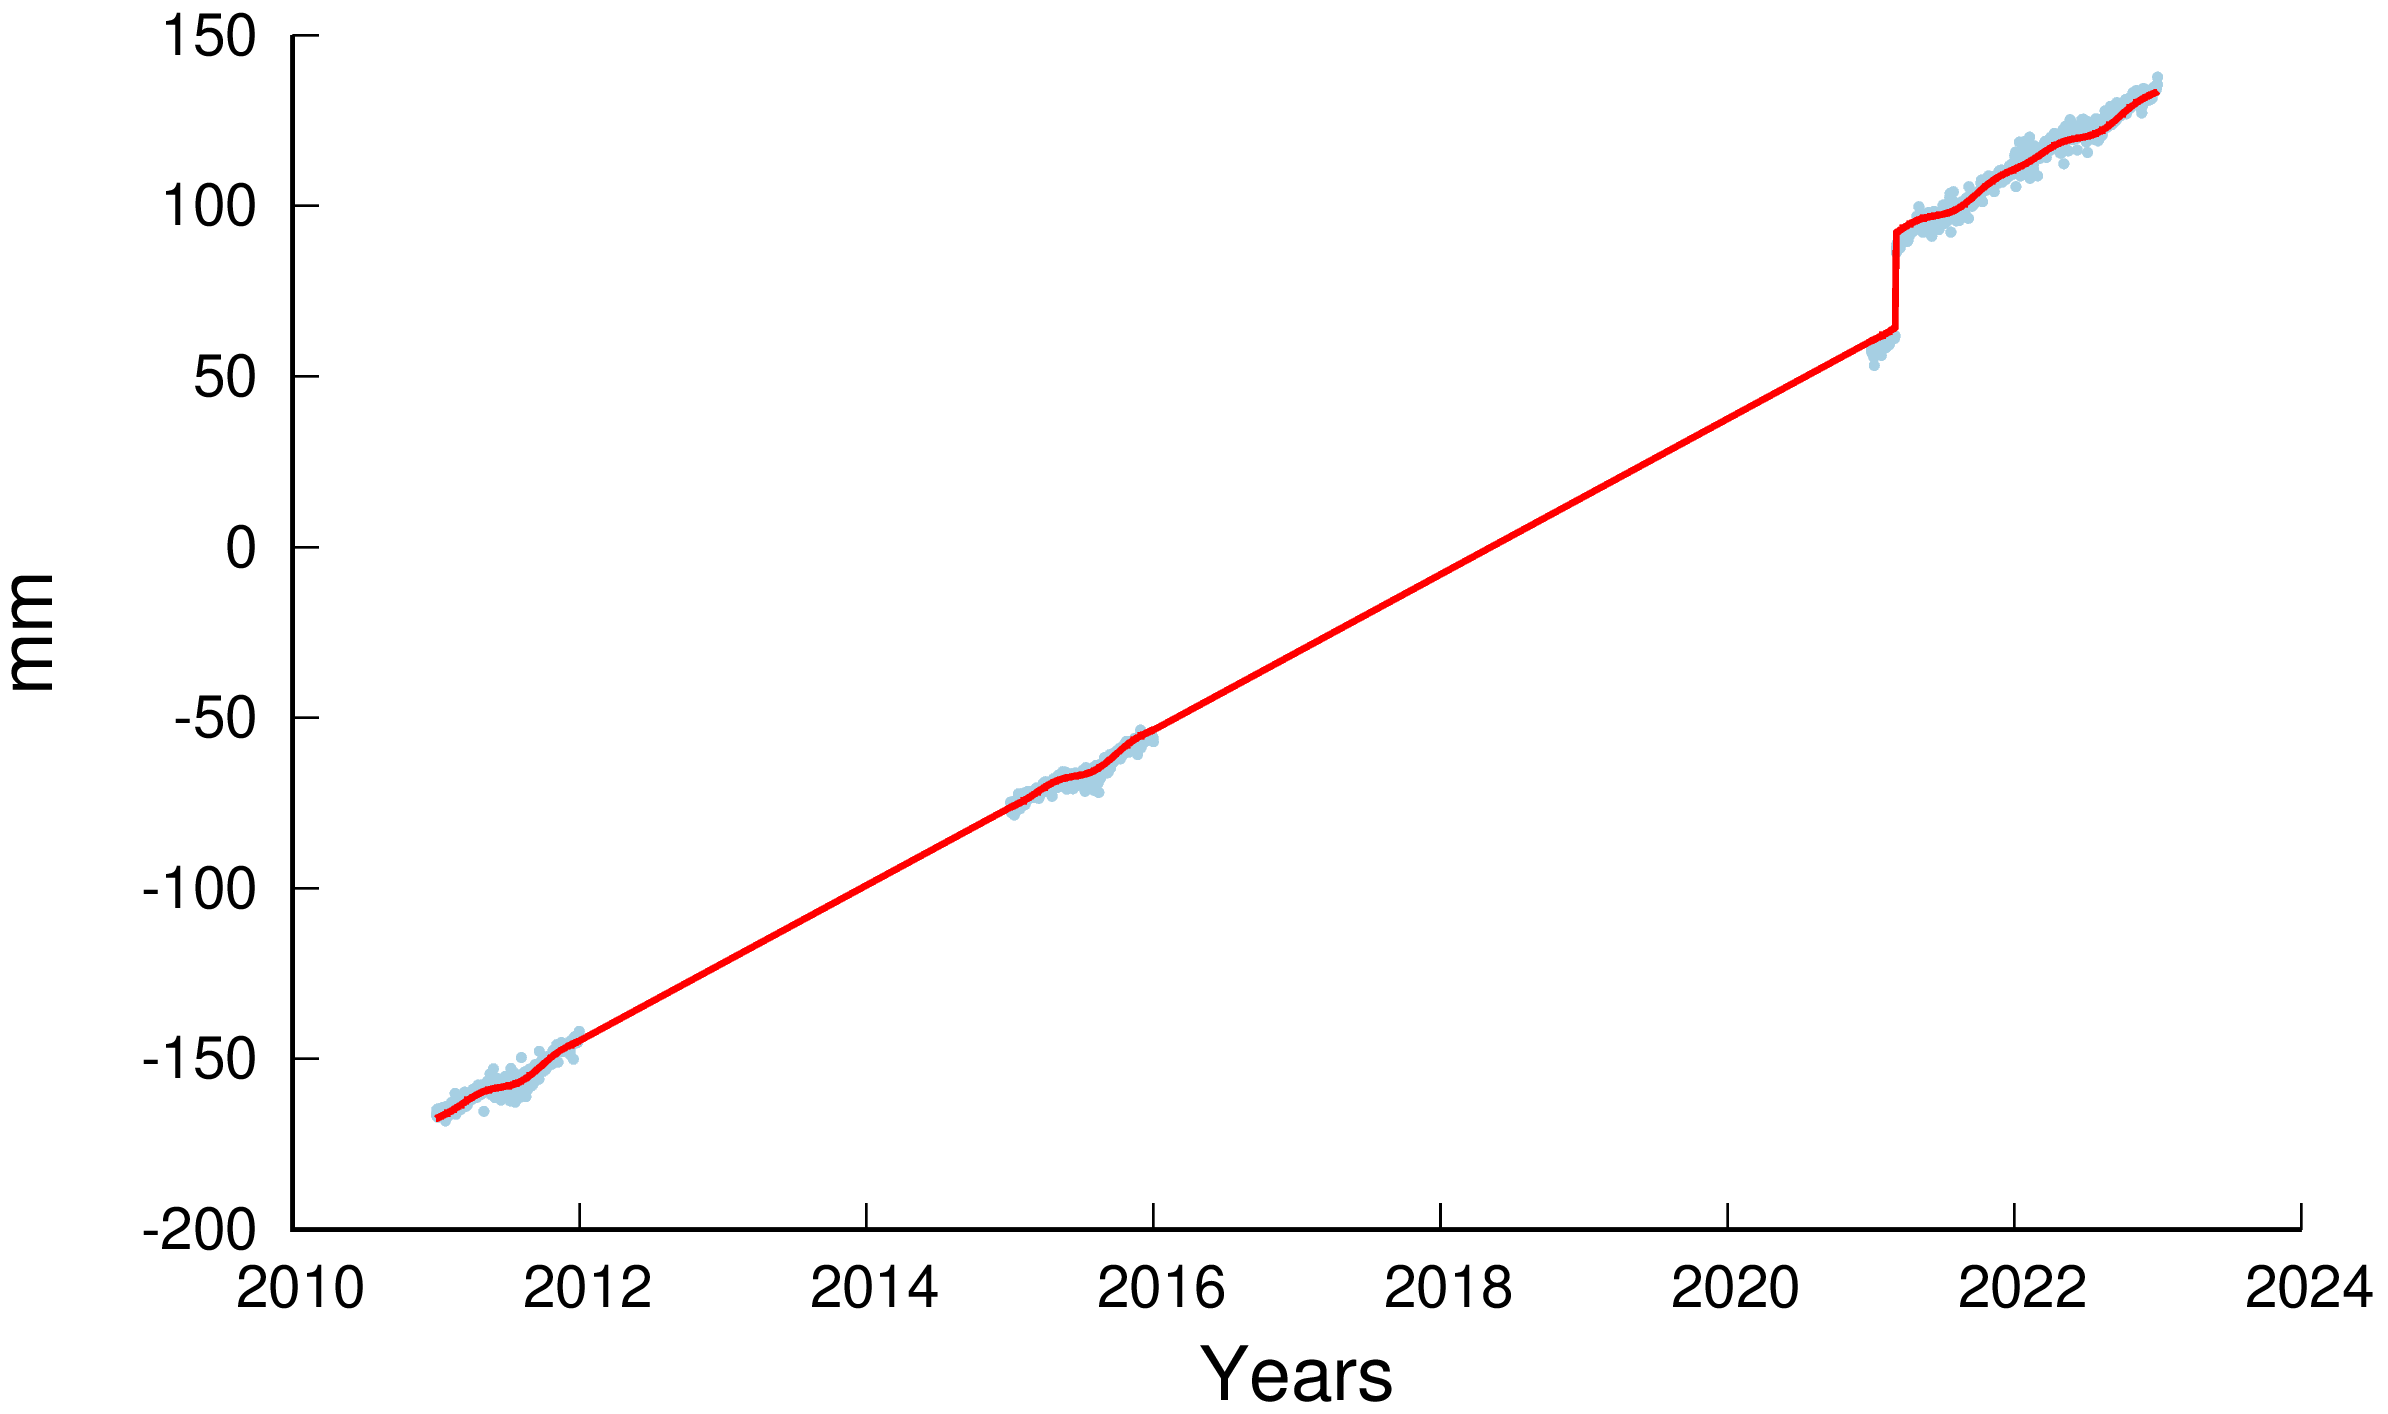
\includegraphics[width=.75\textwidth]{057a_1_data.png}\\
         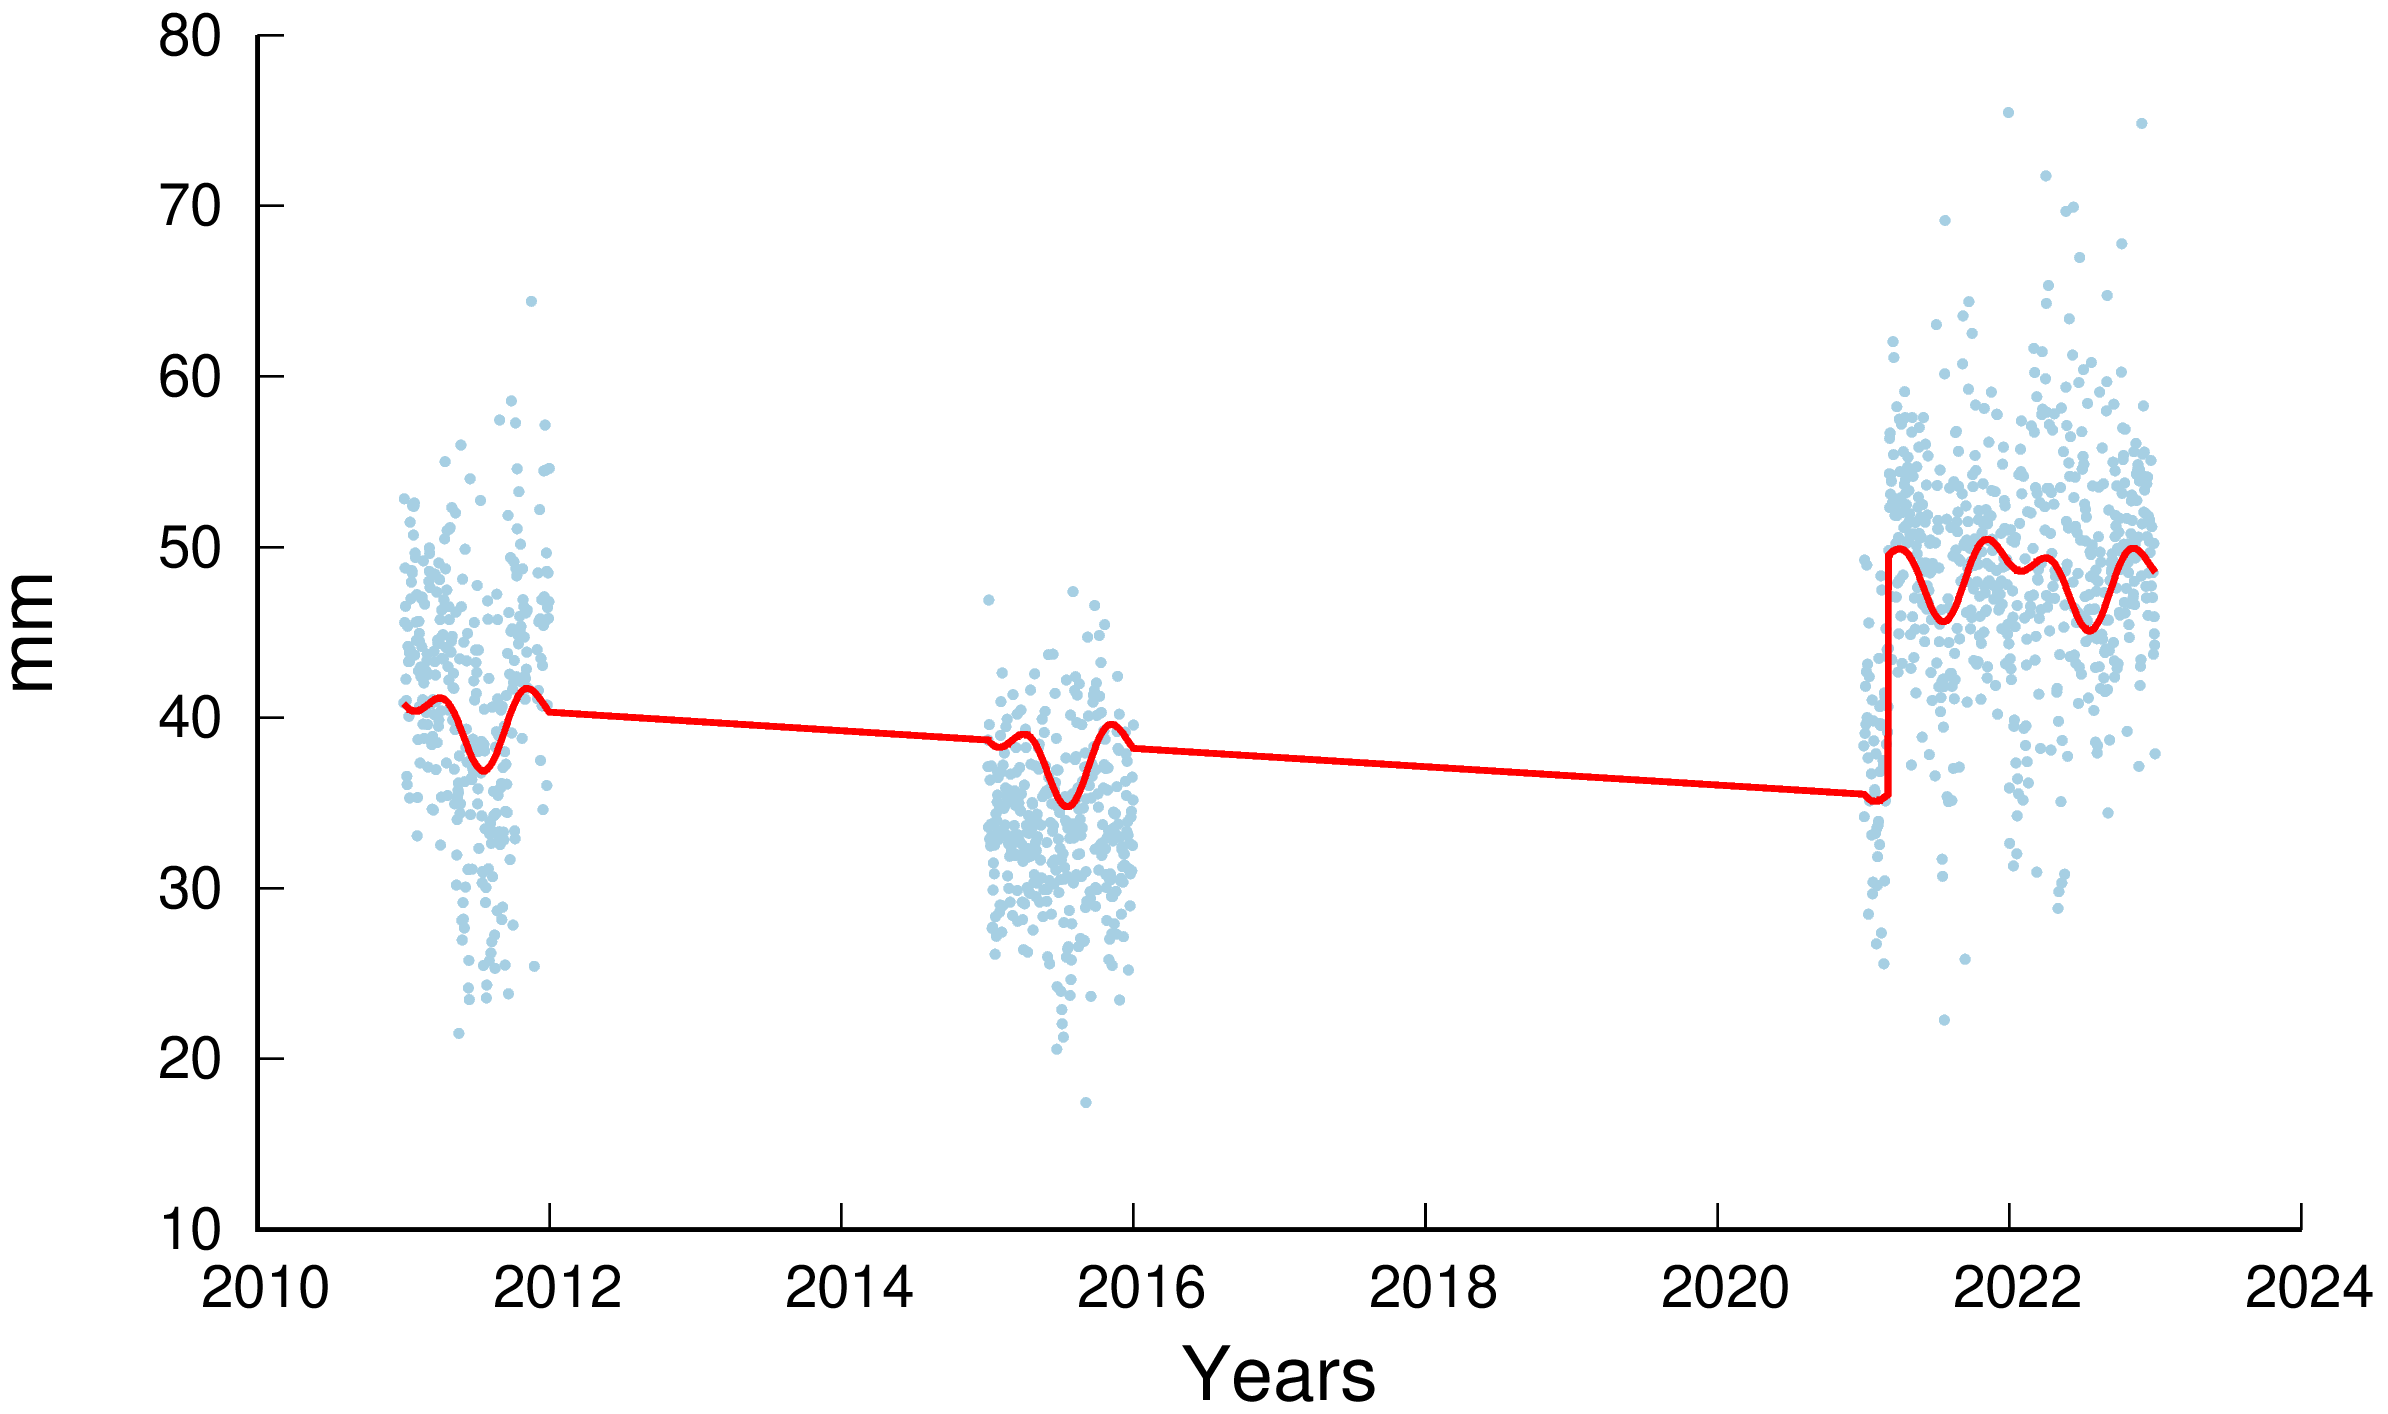
\includegraphics[width=.75\textwidth]{057a_2_data.png}
       \end{center} 
    \end{column}
  \end{columns}
\end{frame}
\note{}

 % ------------------------------------------------------------------------------
\begin{frame}
  \frametitle{Αρμονική ανάλυση}
  \framesubtitle{}
  \label{}

\end{frame}
\note{}

 % ------------------------------------------------------------------------------
\begin{frame}
  \frametitle{Ειδικές περιπτώσεις - Σαντορίνη}
  \framesubtitle{}
  \label{}

\end{frame}
\note{}


 % ------------------------------------------------------------------------------
\begin{frame}
  \frametitle{Προσδιορισμός πεδίου ταχυτήτων}
  \framesubtitle{}
  \label{}

\end{frame}
\note{}

